\documentclass[a4paper, 11pt]{report}

\usepackage[square, numbers, comma, sort&compress]{natbib}
\usepackage{xltxtra}
\usepackage{xgreek}
\usepackage{wrapfig}
\usepackage{graphicx}
\usepackage{caption}
\usepackage[chapter]{algorithm}
\usepackage{algpseudocode}
\usepackage{multirow}
\usepackage{amsmath}
\usepackage{makeidx}
\usepackage{hyperref}
\usepackage{fancyhdr}
\usepackage{paralist}

\newcommand{\HRule}{\rule{\linewidth}{0.5mm}}
\renewcommand{\listalgorithmname}{Κατάλογος αλγορίθμων}

\setmainfont{GFS Neohellenic}

\setlength{\headheight}{15pt}
\pagestyle{fancy}
\rhead{}
\lhead{\nouppercase{\textsc{\leftmark}}}
\renewcommand{\headrulewidth}{0pt}
\makeatletter
\renewcommand{\chaptermark}[1]{\markboth{\textsc{\@chapapp}\ \thechapter:\ #1}{}}
\makeatother

\renewcommand{\algorithmicforall}{\textbf{for each}}
%% ----------------------------------------------------------------
\begin{document}
\begin{titlepage}

\begin{center}


% Upper part of the page
%\includegraphics[width=0.15\textwidth]{./logo}\\[1cm]    

\textsc{\LARGE Πολυτεχνείο Κρήτης\\Τμήμα Ηλεκτρονικών Μηχανικών \& Μηχανικών Η/Υ}\\[1.5cm]

\textsc{\Large Διπλωματική Εργασία}\\[0.5cm]


% Title
\HRule \\[0.4cm]
{ \huge \bfseries Σχεδίαση και Υλοποίηση Ενδιάμεσου Λογισμικού σε P-Grid Δίκτυα Ανεκτικά σε Λάθη}\\[0.4cm]

\HRule \\[1.5cm]

% Author and supervisor
\begin{minipage}{0.4\textwidth}
\begin{flushleft} \large
\emph{Συγγραφέας:} \\
Νικόλας Βουρλάκης
\end{flushleft}
\end{minipage}
\begin{minipage}{0.4\textwidth}
\begin{flushright} \large
\emph{Επιβλέπων:} \\
Βασίλης Σαμολαδάς
\end{flushright}
\end{minipage}

\vfill

% Bottom of the page
{\large \today}

\end{center}

\end{titlepage}


\pagenumbering{roman}
\begin{abstract}
Τα peer-to-peer συστήματα εισάγουν διάφορες προκλήσεις στον σχεδιασμό 
τους. Η πολυπλοκότητα τους μπορεί να αντιμετωπιστεί μέσω μιας καλής 
σχεδίασης. Ωστόσο, πολλά peer-to-peer συστήματα αναπτύσσονται με τρόπο 
που επιλύει το συγκεκριμένο πρόβλημα που αντιμετωπίζουν. Ένα θέμα 
επομένως είναι μια γενίκευση και τυποποίηση τέτοιων αρχιτεκτονικών. 
Ωστόσο, στην σχετική βιβλιογραφία βρίσκουμε λίγες αναφορές που 
ασχολούνται με αυτό το θέμα. Στην παρούσα διπλωματική εργασία, βασικός 
στόχος ήταν η σχεδίαση της αρχιτεκτονικής και η υλοποίηση ενδιάμεσου 
λογισμικού ωφέλιμο για τη δημιουργία συστημάτων που εκμεταλλεύονται το 
peer-to-peer μοντέλο. Η Επιρροή για την σχεδίαση υπήρξαν τα 
υπηρεσιοκεντρικά συστήματα και η θεωρία γύρω από αυτά. Βάσει αυτής της 
αρχιτεκτονικής η προσθήκη νέων πολύπλοκων πρωτοκόλλων απλοποιείται. Η 
οργάνωση που ακολουθούν οι peer του δικτύου είναι αυτή του P-Grid. 
δίκτυο που σχηματίζεται από να είναι ανεκτικό σε λάθη και να συνεχίζει 
να λειτουργεί σωστά υπό την παρουσία αποτυχιών. Ο δεύτερος στόχος της 
εργασίας ήταν η δημιουργία ενός fault-tolerant πρωτοκόλλου βάσει του 
οποίου το σύστημα μπορεί να διατηρήσει την τοπολογία του όχι μόνο στην 
περίπτωση αποτυχιών αλλά και στις μεταβολές που παρουσιάζονται λόγω του 
φαινομένου churn. 
\end{abstract}

\renewcommand{\abstractname}{Eυχαριστίες}
\begin{abstract}
Θα ήθελα να ευχαριστήσω τον επιβλέποντα καθηγητή κ. Βασίλη Σαμολαδά για 
την καθοδήγηση και την βοήθεια που πρόσφερε κατά τη διάρκεια εκπόνησης 
της παρούσας διπλωματικής εργασίας. Επίσης, την οικογένειά μου για την 
υπομονή και υποστήριξη που έδειξαν κατά τη διάρκεια των σπουδών μου.
\end{abstract}

\tableofcontents
\listoffigures
\listofalgorithms
%\listoftables
\newpage

%% ----------------------------------------------------------------
\pagenumbering{arabic}
\pagestyle{headings}

\chapter{Εισαγωγή}
\label{chap:Intro}

TODO: Θέλει ανανέωση.

Την τελευταία δεκαετία έχει σημειωθεί σημαντική πρόοδος σε 
συστήματα που εκμεταλλεύονται την αρχιτεκτονική peer-to-peer.

Ένα δίκτυο ομότιμων (peer-to-peer) $[$παραπομπή$]$ είναι μια 
αρχιτεκτονική βάσει της οποίας κάθε μέλος (peer) έχει ισότιμες 
δυνατότητες με τα υπόλοιπα. Στα αμιγώς peer-to-peer δίκτυα, δεν υπάρχει 
κάποιος κόμβος που να κατευθύνει και να οργανώνει τους peer. Μάλιστα, 
κάθε peer συμμετέχει ισοδύναμα στην οργάνωση και στη λειτουργία του 
δικτύου προσφέροντας μέρος των πόρων του. 

Ένα από τα σημαντικά προβλήματα που συναντάμε σε τέτοιες αρχιτεκτονικές, 
είναι η αστοχία των peer κατά τη διάρκεια ζωής του δικτύου. Ένας peer 
μπορεί να αποτύχει για δυο λόγους, είτε έχει πρόβλημα ο ίδιος (έχει 
κρασάρει κλπ), είτε υπάρχει πρόβλημα στην σύνδεση του. Οπότε σημαντικό 
χαρακτηριστικό είναι να συνεχίσει ένα peer-to-peer σύστημα να λειτουργεί 
σωστά καθώς και οι υπηρεσίες που παρέχονται να είναι διαθέσιμες 
(available). Υπάρχει η ανάγκη ενός πρωτοκόλλου βάσει του οποίου 
προλαμβάνεται το προηγούμενο πρόβλημα. Ένας μηχανισμός, ο οποίος να 
είναι σε θέση να αναγνωρίσει γρήγορα και με ακρίβεια peer που αστοχούν ή 
αποκλίνουν από την αναμενόμενη συμπεριφορά. Γενικά, ένας peer μπορεί να 
μαθαίνει πληροφορίες για τους υπόλοιπους με δυο τρόπους $[$παραπομπή$]$. 
Μπορεί να ρωτήσει απευθείας τους peer που τον ενδιαφέρουν άμεσα, όπως 
αυτοί που είναι αποθηκευμένοι στο routing table του, περιμένοντας κάποια 
απάντηση από αυτούς ως απόδειξη ότι λειτουργούν σωστά. Επίσης, από τη 
στιγμή που κάποιοι peer απλά δρομολογούν τα μηνύματα, δεδομένου ότι δεν 
έχουν φτάσει ακόμα στον τελικό παραλήπτη, μπορεί να γίνει γνωστό στο 
δίκτυο ποιοι peer είναι ενεργοί. Χρησιμοποιώντας αυτές τις πληροφορίες 
οι peer μπορούν να διορθώσουν τις προβληματικές αναφορές. Μεγάλο ρόλο 
παίζει ο χρόνος που χρειάζεται για να αναγνωριστεί μια αστοχία. Όσο πιο 
γρήγορα εντοπιστεί το πρόβλημα τόσο πιο γρήγορα θα διορθωθεί κι άρα το 
δίκτυο ξοδεύει λιγότερους πόρους για να στείλει μηνύματα σε peer που 
έχουν πέσει. Παρόμοια μοντέλα έχουν περιγραφεί στις δημοσιεύσεις 
$[$παραπομπή$]$ και $[$παραπομπή$]$.

Το P-Grid $[$παραπομπή$]$, είναι ένα πρωτόκολλο το οποίο καθορίζει τον 
τρόπο οργάνωσης και αλληλεπίδρασης των peer. Ανήκει στην κατηγορία των 
δομημένων δικτύων ομότιμων (structured peer-to-peer). Οργανώνεται σε ένα 
κατανεμημένο κατακερματισμένο πίνακα (DHT) και η τοπολογία που 
δημιουργεί είναι όμοια με αυτή ενός binary trie. Είναι ένα πλήρως 
αποκεντρωμένο δίκτυο που βασίζεται σε τυχαιοκρατικούς αλγορίθμους για 
την κατασκευή των πινάκων δρομολόγησης (routing table). Τη δεδομένη 
στιγμή, το πρωτόκολλο P-Grid, υλοποιεί ένα αλγόριθμο αντιγραφής 
δεδομένων (replication). Υπάρχουν, συνεπώς, οι κόμβοι οι οποίοι έχουν 
την αρχική πληροφορία και οργανώνουν το DHT και οι κόμβοι οι οποίοι 
αντιγράφουν την πληροφορία και επιλέγονται τυχαία από τους 
προηγούμενους. Με replication επιτυγχάνεται η σταθερότητα του συστήματος 
και μάλιστα αυξάνεται η πιθανότητα να βρεθεί ένα κλειδί, μιας και 
συμμετέχουν στην αναζήτηση όλοι οι peer. Πρέπει, όμως, οι replicated 
peer να συγχρονίζουν διαρκώς τα δεδομένα τους ώστε να έχουμε data 
consistency. Η διαδικασία αυτή στο P-Grid γίνεται ανά τυχαία χρονικά 
διαστήματα. Στη δημοσίευση $[$παραπομπή$]$, αναφέρονται γενικά 
προβλήματα που μπορεί να υπάρξουν με την τεχνική του replication.

Αντίστοιχα, στο Chord $[$παραπομπή$]$ οι peer ανήκουν σε ένα κύκλο 
κρατώντας ο καθένας πληροφορίες για τους successor τους. Κάθε peer 
αποφασίζει ποια είναι η κατάσταση του γείτονά του πχ κάνοντας ping. Σε 
περίπτωση που καταλάβει κάποια αστοχία τότε βρίσκει το νέο successor του 
(διαδικασία stabilization) και διορθώνει κατάλληλα το routing table του. 
Το ζητούμενο είναι να διατηρηθεί ο κύκλος. Δεν έχουμε data consistency 
σε επίπεδο πρωτοκόλλου και η αποτυχία κόμβου ισοδυναμεί με απώλεια 
δεδομένων. Επίσης, ένα άλλο πρόβλημα που προκύπτει όταν έχουμε 
συνεχόμενες αποτυχίες είναι η δημιουργία πολλαπλών κύκλων.

Σε άλλα πρωτόκολλα όπως το Tapestry $[$παραπομπή$]$ έχουμε redundancy. 
Τα μηνύματα ακολουθούν συγκεκριμένο μονοπάτι και κάθε peer αποθηκεύει 
έναν αριθμό από δείκτες προς άλλους peer. Στην περίπτωση αστοχίας ενός 
peer που άνηκε στο μονοπάτι, επιλέγεται ένας από τους προηγούμενους 
δείκτες και προωθείται το μήνυμα εκεί. Εδώ, έχουμε ένα επιπλέον overhead 
για την αποθήκευση των redundant δεικτών καθώς και επιπλέον maintenance.

\chapter{Συστήματα Peer-to-Peer}
\label{chap:P2P}

\section{Εισαγωγή}

Ένα peer-to-peer σύστημα είναι ένα δίκτυο αποτελούμενο από ισότιμους 
συμμετέχοντες, τους peer. Αυτοί διαμοιράζονται τους πόρους που έχει ο 
καθένας μεταξύ τους, όπως υπολογιστική ισχύ ή αποθηκευτικό χώρο. 
Χαρακτηριστικό του συστήματος, που το διαχωρίζει από την κλασική 
αρχιτεκτονική client-server, είναι πως ένας peer είναι πάροχος υπηρεσιών 
και πόρων και την ίδια στιγμή αιτείται αντίστοιχη χρήση από 
απομακρυσμένους peer. Τα peer-to-peer συστήματα χωρίζονται σε δομημένα 
(structured) και μη (unstructured). 

Στα δομημένα peer-to-peer συστήματα η τοπολογία του δικτύου 
κατασκευάζεται ντετερμινιστικά με μια κλασική οργάνωση να είναι οι 
κατανεμημένοι πίνακες κατακερματισμού (DHT). Υπάρχει ένας ευρύτερος 
χώρος αναγνωριστικών από όπου τα δεδομένα και οι peer αντιστοιχούνται σε 
κλειδιά. Ένα σημαντικό ζήτημα του συστήματος είναι για ποια δεδομένα 
είναι υπεύθυνος ένας peer βάσει των κλειδιών τους. Παράδειγμα τέτοιου 
συστήματος είναι το Chord \citep{Tanenbaum2006}. Οι peer οργανώνονται 
πάνω σε ένα κύκλο. Κάθε peer είναι υπεύθυνος για εκείνα τα δεδομένα που 
τους αναλογούν κλειδιά μικρότερα σε σχέση με αυτό του peer. Επίσης, ένας 
peer, με βάση την τοποθεσία του, διατηρεί μια λίστα από γείτονες peer οι 
οποίοι βρίσκονται σε συγκεκριμένες αποστάσεις πάνω στον κύκλο. Το 
αποτέλεσμα αυτής της τοπολογίας του Chord είναι πως ένα lookup 
εξυπηρετείται σε $O(logN)$ βήματα.

Η δεύτερη περίπτωση είναι τα μη δομημένα συστήματα. Αυτά στηρίζονται 
συνήθως σε τυχαιοκρατικούς αλγορίθμους για την κατασκευή της τοπολογίας. 
Δεν υπάρχει ένας συγκεκριμένος σχηματισμός και κάθε peer σχετίζεται με 
γείτονες που έχουν επιλεγεί τυχαία. Μια συνηθισμένη πρακτική σε αυτή την 
κατηγορία συστημάτων είναι η ύπαρξη των υπερκόμβων (supernode). Όσο το 
δίκτυο επεκτείνεται, τόσο περισσότερο αυξάνεται ο χρόνος εξυπηρέτησης 
ενός lookup. Ταυτόχρονα έχουμε και αυξημένη χρήση του bandwidth του 
δικτύου μιας και η πρακτική που ακολουθείται είναι αυτή του flooding. Οι 
υπερκόμβοι λύνουν αυτό το πρόβλημα είτε διατηρώντας ένα ευρετήριο με 
τους πόρους και τους peer του δικτύου είτε λειτουργώντας ως 
διαμεσολαβητές στη δρομολόγηση των μηνυμάτων (broker). Αφού είναι και 
αυτοί μέρος του δικτύου, τότε το σύστημα οδηγείται σε μια ιεραρχική 
δομή.

\section{Το P-Grid Σύστημα}

Το P-Grid 
\citep{Abererb, Aberer, Abererc, Abererd, Aberer2004, Aberer2003, Aberere, Aberer2002} 
είναι ένα πλήρως αποκεντρωμένο και δομημένο 
(structured) peer-to-peer σύστημα. Χρησιμοποιεί τυχαιοκρατικούς 
αλγορίθμους για την κατασκευή και την λειτουργία του. Η τοπολογία που 
δημιουργείται είναι ένα δυαδικό trie δέντρο και χρησιμοποιούνται 
προθέματα κλειδιών για την δρομολόγηση των μηνυμάτων μέσα στο δίκτυο.

Οι peer αποφασίζουν κατά ζεύγη τον τρόπο με τον οποίο θα 
χωρίσουν το χώρο κλειδιών (key space). Κάθε κατάτμηση του χώρου 
αντιστοιχεί σε μια συγκεκριμένη δυαδική συμβολοσειρά ή οποία αποτελεί 
και το μονοπάτι ενός peer. Στο σχήμα \ref{fig:PGrid_overlay} φαίνεται η τελική 
διαμόρφωση του χώρου κλειδιών και της τοπολογίας που έχουν σχηματίσει οι 
peer. Το δίκτυο αποτελείται από τέσσερις peer κάθε ένας εκ των οποίων 
έχει συσχετιστεί με ένα μονοπάτι. Η ρίζα του δέντρου αποτελεί το 
συνολικό χώρο των κλειδιών. Οι διακλαδώσεις σε κάθε ύψος αναπαριστούν 
κατατμήσεις του χώρου ένα ψηφίο τη φορά. Παράδειγμα, μετά τη ρίζα, 
έχουν δημιουργηθεί δύο μεγάλα υπόδεντρα. Το αριστερό περιλαμβάνει όλα τα 
κλειδιά τα οποία έχουν πρόθεμα το \textit{'0'}, ενώ το αριστερό αυτά που έχουν 
πρόθεμα το \textit{'1'}. Συνεπώς, οι peer ανάλογα με το μονοπάτι με το οποίο 
έχουν συσχετιστεί, γνωρίζουν ένα συγκεκριμένο πλήθος κλειδιών.

\begin{figure}[htbp]
\centering
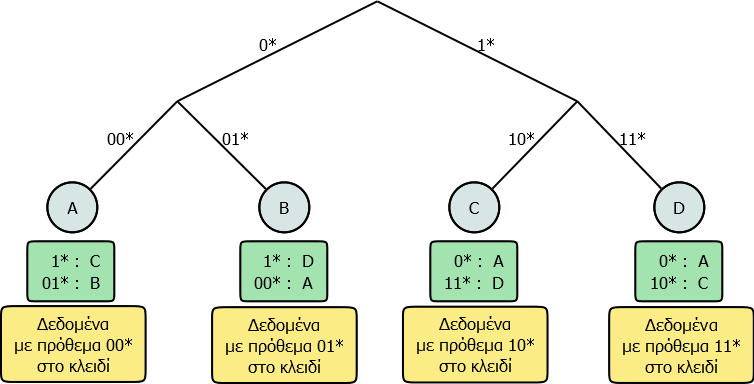
\includegraphics[scale=0.4]{Figures/P2P_PGrid/PGrid_overlay_network.png}
\caption{Η τοπολογία ενός δικτύου P-Grid}
\label{fig:PGrid_overlay}
\end{figure}

Για κάθε επίπεδο του δέντρου, αποθηκεύονται αναφορές στον πίνακα 
δρομολόγησης προς τους peer των οποίων το μονοπάτι ανήκει στο συζυγές 
υπόδεντρο. Παράδειγμα, ο peer Α έχει μονοπάτι \textit{'00'} και επομένως θα 
αποθηκεύσει αναφορές για το επίπεδο με μονοπάτι \textit{'0'} έναν peer από το 
συζυγές του που είναι το υπόδεντρο με μονοπάτι \textit{'1'}. Αντίστοιχα για το 
\textit{'00'} είναι το \textit{'01'}. Στο σχήμα \ref{fig:PGrid_overlay} έχει 
συσχετίσει το \textit{'1'} με τον peer C και το \textit{'01'} με τον B. 
Η επιλογή των peer που θα επιλέξει να κρατήσει αναφορές είναι τυχαία. Επίσης, 
οι peer που αποθηκεύονται ανά επίπεδο μπορεί να είναι περισσότεροι του ενός. 
Βάσει αυτής της τοπολογίας, μια αναζήτηση θα κάνει Ο(logN) βήματα μέχρι να 
βρεθεί το αποτέλεσμα της. Άλλο πλεονέκτημα είναι και η δυνατότητα εκτέλεσης 
αναζητήσεων με δεδομένο ένα εύρος κλειδιών (key range).

Όσον αφορά τα δεδομένα που μπορεί να αποθηκεύσει κάθε peer, 
ακολουθείται η ίδια λογική. Υπάρχει μια συνάρτηση κατακερματισμού η 
οποία αντιστοιχεί κλειδιά σε δεδομένα. Κάθε peer είναι υπεύθυνος για 
εκείνο το κομμάτι των δεδομένων που έχει πρόθεμα το μονοπάτι του.

Τέλος, το σύστημα υποστηρίζει διάφορα πρωτόκολλα. Αυτό που μας 
ενδιαφέρει στην παρούσα εργασία είναι αυτό της ανοχής λαθών 
(fault-tolerance). Αυτό που προτείνεται και είναι ήδη υλοποιημένο είναι 
η τεχνική της αντιγραφής (replication). Κάθε μονοπάτι του δέντρου 
αντιστοιχεί σε πολλαπλούς peer. Αυξάνει τη γενική αντοχή του συστήματος 
σε αποτυχίες peer. Το κόστος είναι η μείωση της χωρητικότητας του 
δικτύου, αφού μέρος των peer είναι αντίγραφα άλλων. Επίσης γίνεται πιο 
πολύπλοκη η διατήρηση και ο συγχρονισμός του συστήματος. 

\chapter{Σχετική Εργασία και Θεωρία στην Αρχιτεκτονική} 
\label{chap:Literature}

\section{Σχετική Εργασία}

Τα τελευταία χρόνια γίνεται μια προσπάθεια να τυποποιηθούν τα 
peer-to-peer συστήματα σε μια ενιαία αρχιτεκτονική. Πιο γενικά χρειάζεται ένα 
μοντέλο αναφοράς όπου περιγράφονται βασικές οντότητες και 
αλληλεπιδράσεις και βάσει αυτού μπορούν να κατασκευαστούν τέτοια 
συστήματα.

\begin{wrapfigure}{L}{0.5\textwidth}
  \begin{center}
    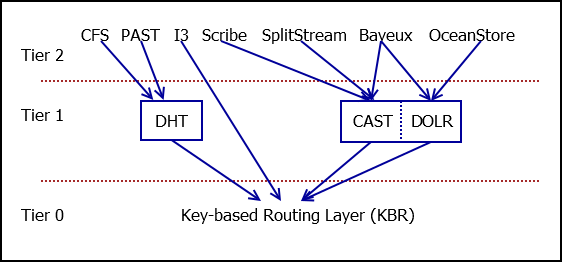
\includegraphics[width=0.48\textwidth]{Figures/Related_work/Towards_a_common_API_(tiers).png}
  \end{center}
  \caption{Towards a common API}
  \label{fig:Α_common_API}
\end{wrapfigure}
Στη δημοσίευση \citep{F.Dabek2003} έχουμε το διαχωρισμό του συστήματος 
σε τρία επίπεδα. Το πρώτο επίπεδο αφορά τη δρομολόγηση, η οποία βασίζεται σε κλειδιά 
(key-based routing). Πάνω σε αυτό χτίζονται τα πρωτόκολλα του συστήματος, 
όπως κατανεμημένοι πίνακες κατακερματισμού (DHT), αποκεντρωμένη 
τοποθεσία αντικειμένου και δρομολόγησης (Decentralized Object Location 
and Routing) καθώς και anycast/multicast λειτουργικότητα. Οι εφαρμογές 
έχουν πρόσβαση που αποτελούν το ανώτερο αρχιτεκτονικό επίπεδο, έχουν 
πρόσβαση απευθείας στα δυο κατώτερα επίπεδα. Οι διεπαφές που 
προτείνονται όμως δεν μπορούν να καλύψουν όλες τις ανάγκες. Στο σχήμα  
\ref{fig:Α_common_API} φαίνονται τα επίπεδα της προτεινόμενης αρχιτεκτονικής.

\begin{wrapfigure}{L}{0.45\textwidth}
  \begin{center}
    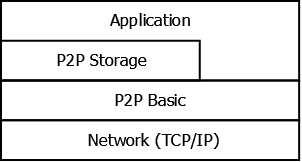
\includegraphics[width=0.43\textwidth]{Figures/Related_work/The_essence_of_p2p_(architecture).png}
  \end{center}
  \caption{Προτεινόμενη αρχιτεκτονική από Aberer et al.}
  \label{fig:Essence}
\end{wrapfigure}

Ο εμπνευστής του P-Grid συστήματος με την ομάδα του εισάγει ένα 
μοντέλο αναφοράς \citep{Aberer05theessence} στο οποίο μπορούν να σχεδιαστούν 
διάφορα peer-to-peer συστήματα. Στο σχήμα \ref{fig:Essence} παρουσιάζονται τα 
αρχιτεκτονικά επίπεδα του μοντέλου. Στηρίζεται πάνω στο επίπεδο του 
δικτύου το οποίο συγκεντρώνει τα πρωτόκολλα 
TCP/IP. Αυτό παρέχει τις λειτουργίες του στο βασικό επίπεδο (P2P basic) το οποίο και υλοποιεί το 
peer-to-peer δίκτυο. Οι λειτουργίες που παρέχει είναι η σύνδεση (join) 
και η αποχώρηση (leave) στο δίκτυο, αναζήτησης (lookup) και δρομολόγησης 
(route). 
Στη συνέχεια έχουμε το επίπεδο αποθήκευσης (P2P storage) που 
παρέχει λειτουργίες εισαγωγής (insert), διαγραφής (delete), ανανέωσης 
(update) δεδομένων στο δίκτυο καθώς και τη διενέργεια ερωτήσεων πάνω σε 
αυτά (query). Για την ανάπτυξη μιας εφαρμογής, χρησιμοποιούνται οι 
διεπαφές που προσφέρονται από το βασικό επίπεδο και αυτό της 
αποθήκευσης. Στο σχήμα \ref{fig:Essence_UML} παρουσιάζεται το 
προτεινόμενο βασικό μοντέλο.

Σε αυτό φαίνονται τα απαραίτητα συστατικά που προκύπτουν από την 
ανάλυση, οι διάφοροι περιορισμοί που τίθενται και οι διεπαφές που πρέπει 
να υποστηρίζει κάθε peer-to-peer σύστημα. Στην υλοποίηση του P-Grid 
\footnote{\url{http://www.p-grid.org}}
από τον Schmidt \citep{Schmidt2007}, ακολουθήθηκε το παραπάνω 
μοντέλο. Η όλη λογική είναι ένα peer-to-peer σύστημα να είναι χαλαρά 
συνδεδεμένο με τις υπηρεσίες που προσφέρουν το βασικό επίπεδο και αυτό 
της αποθήκευσης. Στόχος είναι η ευκολία αλλαγής συμπεριφοράς του ίδιου 
συστήματος εναλλάσσοντας τις διάφορες υλοποιήσεις. Παρόλα αυτά όπως 
προκύπτει από την εξέταση της υλοποίησης, είναι δύσκολο να επεκταθεί μια 
υπάρχουσα υλοποίηση με άλλα πρωτόκολλα πιο πολύπλοκα.

\begin{figure}[htpb]
  \begin{center}
    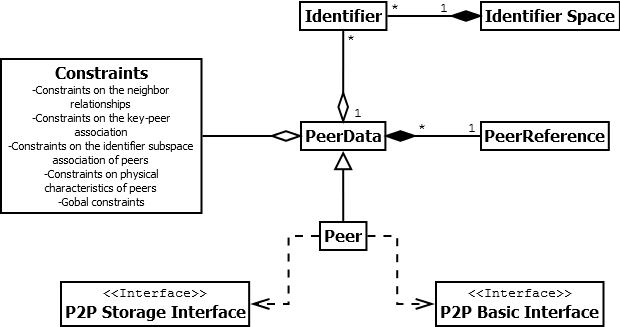
\includegraphics[scale=0.55]{Figures/Related_work/The_essence_of_p2p_(uml).png}
  \end{center}
  \caption{Προτεινόμενο μοντέλο αναφοράς από Aberer et al.}
  \label{fig:Essence_UML}
\end{figure}

\begin{wrapfigure}{L}{0.5\textwidth}
  \begin{center}
    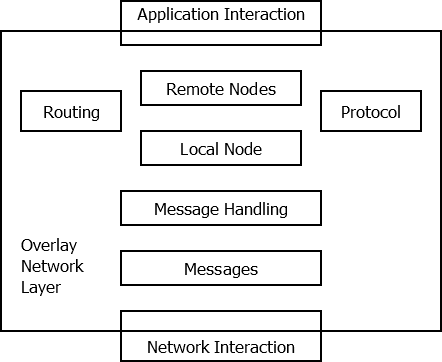
\includegraphics[width=0.48\textwidth]{Figures/Related_work/A_pattern_language.png}
  \end{center}
  \caption{A Pattern Language}
  \label{fig:Patterns}
\end{wrapfigure}

Για την εσωτερική δομή επιπέδων, όπως αυτό του βασικού της παραπάνω 
αρχιτεκτονικής , συντελείται μια προσπάθεια να δημιουργηθούν σχεδιαστικά 
πρότυπα. Στις δημοσιεύσεις \citep{Grolimund2005, Grolimund2006} αναλύονται 
ένα σύνολο peer-to-peer συστημάτων και ενδιάμεσου λογισμικού. Από αυτό 
προκύπτουν σχεδιαστικά πρότυπα που έχουν να κάνουν με ένα βασικό στοιχείο 
αυτών των συστημάτων που είναι η δρομολόγηση των μηνυμάτων μέσα στο δίκτυο. 
Στο σχήμα \ref{fig:Patterns} φαίνεται η αρχιτεκτονική δομή του συγκεκριμένου επιπέδου. 
Κάθε στοιχείο του επιπέδου περιλαμβάνει μια σειρά σχεδιαστικών προτύπων. 

Στη δημοσίευση \citep{Amoretti2005} εισάγεται η έννοια 
του Peer ως σχεδιαστικό πρότυπο. Το πρόβλημα που προσπαθεί να επιλυθεί 
είναι η αποτελεσματική κατανομή του φόρτου εργασίας και η υψηλή 
διαθεσιμότητα των πόρων. Η λογική είναι παρόμοια, μόνο που πλέον οι πόροι 
και οι λειτουργίες που προσφέρει ένας peer παρουσιάζονται ως υπηρεσίες. 
Ενδιαφέρει ο τρόπος με τον οποίο περιγράφονται οι υπηρεσίες και 
προτείνεται η ύπαρξη είτε μιας WSDL διεπαφής όπου μπορεί να ανακτηθεί 
πλήρως η λειτουργικότητά της είτε OWL-S περιγραφών σε περίπτωση που 
είναι αναγκαία η σημασιολογική περιγραφή (semantic) της πληροφορίας. 
Προτείνεται, μάλιστα, η χρήση Web Service αρχιτεκτονικής δεδομένου των 
πλεονεκτημάτων που μπορεί να φέρει μια τέτοια υπηρεσία. 

Από την πρακτική εφαρμογή του προτύπου προκύπτει ένα πλαίσιο ανάπτυξης 
peer-to-peer συστημάτων, το SP2A \citep{Amoretti2005SP2A}. 
Χρησιμοποιήθηκαν τεχνολογίες όπως η JXTA και Web Services. Για την ανάπτυξη 
των τελευταίων χρησιμοποιήθηκαν τα JXTA-SOAP και OWL-S. Η περιγραφή των web 
service μέσω OWL-S κάνει εύκολη την ανακάλυψη, την εκτέλεση, την σύνθεση 
αυτών και την παρακολούθησή τους (monitoring). Παρόλα αυτά, το συγκεκριμένο 
framework υποστηρίζει υβριδικά και καθαρά peer-to-peer δίκτυα χωρίς όμως να 
υπάρχει συγκεκριμένη τοπολογία. Επίσης, δεν υπάρχει η έννοια της 
σύνθεσης των υπηρεσιών στο ίδιο το λογισμικό του peer σε πιο πολύπλοκες 
διαδικασίες/πρωτόκολλα.

Σημαντική δουλειά είναι τα JXTA πρωτόκολλα \citep{JXTA2007}. Αυτά 
αποτελούν μια ανοιχτή διαδικτυακή πλατφόρμα για peer-to-peer συστήματα. 
Τυποποιείται ο τρόπος με τον οποίο ένας peer ανακαλύπτει άλλους, το πώς 
οργανώνεται σε ομάδες peer και πώς επικοινωνεί. Επίσης, ορίζονται 
πρωτόκολλα για τη διαφήμιση και ανακάλυψη διαδικτυακών πόρων. Υπάρχουν 
τρία αρχιτεκτονικά επίπεδα, με πρώτο το επίπεδο της πλατφόρμας όπου 
ορίζονται κλασικοί τύποι για ένα peer-to-peer δίκτυο. Στη συνέχεια, 
έχουμε το επίπεδο των υπηρεσιών το οποίο περιλαμβάνει διαδικτυακές 
υπηρεσίες, όπως αναζήτησης και ευρετηριοποίησης, αποθηκευτικού χώρου, 
διαμοιρασμού αρχείων, κατανεμημένα συστήματα αρχείων και άλλα. Το τελικό 
επίπεδο είναι αυτό της εφαρμογής που εκμεταλλεύεται τις προσφερόμενες 
υπηρεσίες. Δεν υπάρχει όμως καθορισμός της τοπολογίας των peer-to-peer 
δικτύων που προκύπτουν. Επιπλέον, τα πρωτόκολλα είναι ορισμένα ως ένα σύνολο 
από XML μηνύματα προκειμένης της ανεξαρτητοποίησης από λειτουργικά 
συστήματα και γλώσσες προγραμματισμού.

\section[Υπηρεσιοκεντρική Αρχιτεκτονική]{Υπηρεσιοκεντρική Αρχιτεκτονική (Service - Oriented Architecture - SOA)}
\label{sec:SOA}

\subsection{Η Υπηρεσία ως Δομικό Στοιχείο}

Η αρχιτεκτονική που εισάγουμε έχει επηρεαστεί από τα συστήματα που 
ακολουθούν το μοντέλο της υπηρεσιοκεντρούς αρχιτεκτονικής (SOA). Θα 
ακολουθήσει μια μικρή ανάλυση τέτοιων συστημάτων και των χαρακτηριστικών 
τους πριν την εξήγηση της αρχιτεκτονικής. Θα δούμε γιατί η έννοια της 
υπηρεσίας και της θεωρίας που έχει αναπτυχθεί είναι χρήσιμη και ποιά 
είναι τα πλεονεκτήματα που απορρέουν από μια τέτοια σχεδίαση. To 
υπηρεσιοκεντρικό μοντέλο είναι ένα πρότυπο για την οργάνωση και τη χρήση 
κατανεμημένων λειτουργιών \citep{OASIS-soa-rm}. 

Στο σχήμα \ref{fig:SOA_layers} παρουσιάζονται τα αρχιτεκτονικά επίπεδα ενός 
υπηρεσιοκεντρικού συστήματος \citep{Bianco2011}. Τα επίπεδα όπως παρουσιάζονται είναι:

\begin{figure}[htbp]
  \begin{center}
    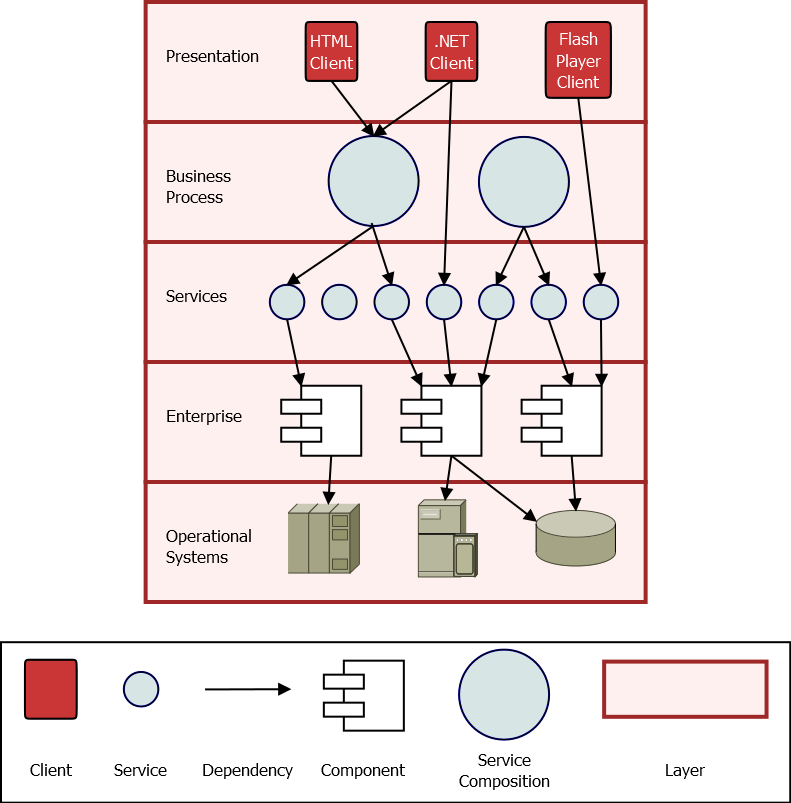
\includegraphics[scale=0.3]{Figures/SOA/SOA_layers.png}
  \end{center}
  \caption{Αρχιτεκτονικά επίπεδα ενός υπηρεσιοκεντρικού συστήματος}
  \label{fig:SOA_layers}
\end{figure}

\newcounter{numberedCntF}
\begin{enumerate}
\setcounter{enumi}{\thenumberedCntF}
\item \textbf{Business Process.} Οι υπηρεσίες που παρέχονται στο 
επίπεδο των υπηρεσιών, συνήθως συντίθενται σε ροές εργασίας (workflow) 
και βοηθούν στην ανάπτυξη εφαρμογών.
\item \textbf{Services.} Στο επίπεδο αυτό υπάρχουν οι υπηρεσίες. Η 
κλήση των υπηρεσιών καθορίζεται είτε κατά τη διάρκεια της σχεδίασης είτε 
μέσω μιας υπηρεσίας μητρώου (service registry) κατά τη διάρκεια 
εκτέλεσης.
\item \textbf{Enterprise.} Τα διάφορα κομμάτια που ανήκουν στο επίπεδο 
περιέχουν κώδικα που εξυπηρετεί τις ανάγκες των υπηρεσιών. Επίσης, 
παρέχεται πρόσβαση στα συστήματα που βρίσκονται στο κατώτερο επίπεδο.
\item \textbf{Operational Systems.} Εδώ ανήκουν όλα τα λειτουργικά 
εμπορικά και μη συστήματα.
\setcounter{numberedCntF}{\theenumi}
\end{enumerate}

Η δομική μονάδα του μοντέλου είναι η υπηρεσία. Η υπηρεσία είναι ένας 
μηχανισμός με τον οποίο επιτρέπεται πρόσβαση σε μια ή περισσότερες 
λειτουργίες. Η πρόσβαση παρέχεται μέσω μιας προκαθορισμένης διεπαφής και 
χρησιμοποιείται σύμφωνα με τους περιορισμούς και τις πολιτικές που 
ορίζονται από την περιγραφή της υπηρεσίας. Σύμφωνα με το αρχιτεκτονικό 
μοντέλο της OASIS \citep{OASIS-soa-raf} 
έχουμε διάφορους ρόλους σε μια υπηρεσία. Έχουμε 
αυτόν που προσφέρει την υπηρεσία και ονομάζεται Service Provider. 
Υπάρχει αυτός που ζητά την υπηρεσία για να την 
χρησιμοποιήσει/καταναλώσει και ονομάζεται Service Consumer. Έχουμε τον 
ρόλο του διαμεσολαβητή ο οποίος διευκολύνει την αλληλεπίδραση και τη 
συνδεσιμότητα στην προσφορά και χρήση της υπηρεσίας και ονομάζεται 
Service Mediator. Καταλήγοντας, έχουμε τον κάτοχο της υπηρεσίας ο οποίος 
ονομάζεται Service Owner.

Η κλήση μιας υπηρεσίας έχει το αποτέλεσμα είτε της επιστροφής 
πληροφορίας αν η αίτηση είχε τέτοιο σκοπό είτε της αλλαγής της 
κατάστασης του συστήματος. Σε καμία περίπτωση τον καταναλωτή της 
υπηρεσίας δεν τον ενδιαφέρει ο τρόπος παραγωγής της πληροφορίας ή πως 
έγινε η αλλαγή της κατάστασης. Επιπλέον, δεν γνωρίζει πώς υλοποιείται η 
υπηρεσία που χρησιμοποιεί. Παρακάτω αναφέρονται οι γενικές σχεδιαστικές 
αρχές που διέπουν μια υπηρεσία.

\subsection{Χαρακτηριστικά Υπηρεσιών}

Συνολικά έχουμε δυο κατηγορίες αρχών \citep{Duggan2012}. Η πρώτη 
περιλαμβάνει τις αρχές που αφορούν τα σχεδιαστικά χαρακτηριστικά των 
υπηρεσιών. Αυτά είναι:

\newcounter{numberedCntI}
\begin{enumerate}
\item Τυποποιημένη σύμβαση υπηρεσίας (service contract)
\item Επαναχρησιμοποίηση υπηρεσίας (Service reusability)
\item Αυτονομία υπηρεσίας (Service autonomy)
\item Υπηρεσία χωρίς κατάσταση (Service statelessness)
\item Δυνατότητα ανακάλυψης υπηρεσίας (Service discoverability)
\setcounter{numberedCntI}{\theenumi}
\end{enumerate}

Η δεύτερη κατηγορία περιλαμβάνει τις αρχές που ρυθμίζουν τον τρόπο με 
τον οποίο θα εφαρμοστούν οι παραπάνω αρχές. Αυτές είναι:

\newcounter{numberedCntJ}
\begin{enumerate}
\item Χαλαρή σύνδεση (Service loose coupling)
\item Αφαιρετικότητα (Service abstraction)
\item Δυνατότητα σύνθεσης (Service composability).
\setcounter{numberedCntJ}{\theenumi}
\end{enumerate}
Στη συνέχεια αναλύονται εκείνες οι αρχές που έχουν νόημα για το επίπεδο 
και το μέγεθος του συστήματος που χτίζουμε.

\subsubsection{Τυποποιημένη σύμβαση υπηρεσίας}

Είναι πολύ σημαντικό και αναγκαίο η ύπαρξη σαφών και καλώς 
ορισμένων συμβάσεων και διεπαφών που ενθυλακώνουν τα στοιχεία και τις 
λειτουργίες του συστήματος. Οι πόροι που προσφέρονται από μια υπηρεσία 
πρέπει να διαχειρίζονται μέσω αυτών των συμβάσεων. Δεν πρέπει δηλαδή να 
υπάρχει απευθείας σύνδεση των καταναλωτών της υπηρεσίας με τους 
υποκείμενους πόρους της. Η ανάγκη μας οδηγεί σε αυτή την αρχή είναι η 
χαλαρή συνδεσιμότητα μεταξύ της υπηρεσίας και του χρήστη της. 

Ο καταναλωτής της υπηρεσίας κατ' επέκταση δεσμεύεται από την σύμβαση 
αυτή προκειμένου να έχει πρόσβαση στην υπηρεσία. Η δέσμευση υπάρχει σε 
τέσσερα σημεία:

\newcounter{numberedCntBA}
\begin{enumerate}
\item Την περιγραφή των λειτουργιών που προφέρει η υπηρεσία.
\item Την περιγραφή του μοντέλου των δεδομένων που θα χρησιμοποιηθεί για 
την ανταλλαγή δεδομένων μεταξύ υπηρεσίας και χρήστη.
\item Θέματα που αφορούν την ποιότητα των παρεχόμενων υπηρεσιών (QoS)
\item Τον καθορισμό του τρόπου σύνδεσης του χρήστη με την υπηρεσία.
\setcounter{numberedCntBA}{\theenumi}
\end{enumerate}

\subsubsection{Επαναχρησιμοποίηση υπηρεσίας}

Το να είναι επαναχρησιμοποιήσιμη μια μονάδα λογισμικού είναι 
πολύ σημαντικό χαρακτηριστικό. Τα κατάλληλα επίπεδα αφαιρετικότητας 
βοηθούν στο να επιτευχθεί η αρχή αυτή.

\subsubsection{Αυτονομία υπηρεσίας}

Οι υπηρεσίες που προσφέρει το σύστημα πρέπει να είναι αυτόνομες 
μεταξύ τους. Η σχεδίαση αυτών πρέπει να γίνει με τέτοιο τρόπο ώστε να 
αποφευχθεί οποιαδήποτε επικάλυψη λειτουργικότητας μεταξύ τους. Επίσης, 
οι υπηρεσίες πρέπει να είναι αξιόπιστες ώστε να έχει νόημα η 
επαναχρησιμοποίηση τους. Για να επιτευχθεί αυτό η υπηρεσία έχει τον 
πλήρη έλεγχο στο πώς λειτουργεί. Εξωτερικοί-απομακρυσμένοι πόροι στους 
οποίους δεν υπάρχει έλεγχος δεν πρέπει να επηρεάζουν αρνητικά. 

\subsubsection{Υπηρεσία χωρίς κατάσταση}

Το να μην αποθηκεύεται κατάσταση σε μια υπηρεσία είναι θεμιτό 
αφού προωθεί την επαναχρησιμοποίηση της.

\subsubsection{Χαλαρή σύνδεση}

Τα κίνητρα πίσω από αυτήν την αρχή είναι η δυνατότητα 
επαναχρησιμοποίησης και συντήρησης. Ανεξάρτητες μονάδες λογισμικού 
καλύπτουν εύκολα αυτά τα χαρακτηριστικά. Όσο πιο σφιχτά συνδεδεμένα 
είναι τα στοιχεία του συστήματος όσον αφορά λειτουργικές εξαρτήσεις, 
τόσο περισσότερο αυξάνει η πιθανότητα να εξαπλωθεί και να επηρεάσει μια 
αλλαγή \citep{Meyer1994}. Το μειονέκτημα που εισάγεται όμως, είναι η 
προσθήκη επιπλέον επιπέδων αφαιρετικότητας με τις όποιες συνέπειες που 
έχει αυτό στην απόδοση του συστήματος.

\subsubsection{Αφαιρετικότητα}

Για να υλοποιηθεί σωστά η σύμβαση που προσφέρει η υπηρεσία, η 
σχεδίαση πρέπει να έχει τα απαραίτητα επίπεδα αφαιρετικότητας. 
Παράδειγμα, στη σύνδεση μεταξύ του παρόχου μιας υπηρεσίας και του 
καταναλωτή της διαμεσολαβεί η σύμβαση/διεπαφή αυτής. Αυτό έχει ως 
συνέπεια την απομόνωση εκείνου του κομματιού της υπηρεσίας, όπως είναι η 
υλοποίησή της, το οποίο δεν αποτελεί χρήσιμη γνώση στον χρήστη της. 

Υπάρχουν και άλλα σημεία στο σύστημα που επωφελούνται από αυτή 
την αρχή. Η πλατφόρμα, τα διάφορα πρωτόκολλα, τα δεδομένα και η δομή 
τους αποτελούν όλα διαφορετικά επίπεδα αφαρετικότητας.

\subsubsection{Δυνατότητα σύνθεσης}

Οι υπηρεσίες είναι σχεδιασμένες έτσι ώστε να μπορούν να 
συνδυαστούν και να προκύψουν διαδικασίες που έχουν νόημα για την 
εφαρμογή. Στα υπηρεσιοκετρικά συστήματα η σύνθεση μπορεί να επιτευχθεί 
με την ενορχήστρωσης όπου υπάρχει ένας καθοδηγητής που καθορίζει τον 
ρόλο της κάθε υπηρεσίας. Μπορεί να γίνει επίσης με την χορογραφία όπου 
κάθε υπηρεσία παίζει τον ρόλο της παράγοντας και εκδίδοντας γεγονότα που 
προκύπτουν κατά την εκτέλεσή της και λαμβάνει τα απαραίτητα γεγονότα για 
να επιτελέσει τον ρόλο της.

\chapter{Γενική Δομή Αρχιτεκτονικής}
\label{chap:Arch}

\section{Επίπεδα Συστήματος}

Με οδηγό το υπηρεσιοκεντρικό μοντέλο που περιγράφηκε στην ενότητα
\ref{sec:SOA}, το σύστημα δομείται σε αρχιτεκτονικά επίπεδα. Όπως 
αναφέρθηκε ένα SOA σύστημα χωρίζεται σε:

\newcounter{numberedCntA}
\begin{enumerate}
\item \textbf{Presentation.} Αφορά εφαρμογές που χρησιμοποιούν το σύστημα.
\item \textbf{Business Process.} Εκτελεί συγκεκριμένη λειτουργία που 
έχει να κάνει με τον τύπο της εφαρμογής και συντίθεται από τις 
υπάρχουσες υπηρεσίες.
\item \textbf{Services.} Συμπεριλαμβάνει όλες τις υπηρεσίες.
\item \textbf{Enterprise.} Εξυπηρετεί απευθείας τις ανάγκες των 
υπηρεσιών και προσφέρει πρόσβαση στα συστήματα της επιχείρησης.
\item \textbf{Operational Systems.} Αποτελείται από τις υπάρχουσα 
εμπορικά και μη εξωτερικά συστήματα ή κάποιο συνδυασμό αυτών.
\setcounter{numberedCntA}{\theenumi}
\end{enumerate}

\begin{figure}[htbp]
  \begin{center}
    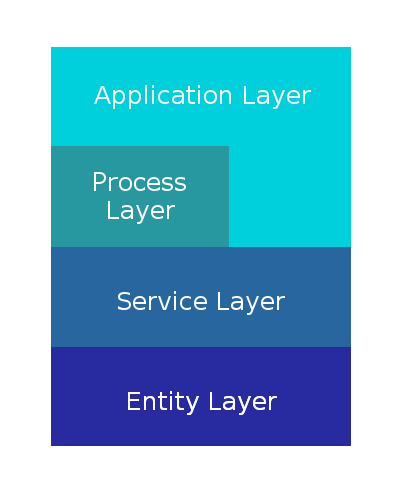
\includegraphics[scale=0.35]{Figures/Architecture/Layers.png}
  \end{center}
  \caption{Τα επίπεδα της αρχιτεκτονικής}
  \label{fig:Layers}
\end{figure}

Με βάση την παραπάνω κατηγοριοποίηση το σύστημα χωρίζεται σε τέσσερα 
επίπεδα. Ξεκινώντας από την κορυφή όπως φαίνεται στο σχήμα 
\ref{fig:Layers} έχουμε:

\begin{itemize}
\item \textbf{Επίπεδο Εφαρμογής (Application Layer).} Το επίπεδο αυτό 
περιλαμβάνει την λογική οποιασδήποτε εφαρμογής που χρησιμοποιήσει την 
παρούσα αρχιτεκτονική. Δεν αφορά την προκείμενη αρχιτεκτονική.
\item \textbf{Επίπεδο Διαδικασιών (Process Layer).} Το επίπεδο αυτό 
περιέχει όλες τις διαδικασίες που στην ουσία είναι συνδυασμός υπηρεσιών 
ώστε να παράγουν ουσιώδεις λειτουργίες προς διευκόλυνση της ανάπτυξης 
εφαρμογών. Στην ουσία οι διαδικασίες είναι κι αυτές υπηρεσίες.
\item \textbf{Επίπεδο Υπηρεσιών (Service Layer).} Το επίπεδο των 
υπηρεσιών περιλαμβάνει ένα σύνολο από διαφορετικές υπηρεσίες. Με τον όρο 
υπηρεσία (service) αναφερόμαστε σε όλες τις σαφώς οριζόμενες και 
αυτόνομες λειτουργίες που έχουν νόημα για ένα peer-to-peer σύστημα. 
Είναι στην ουσία αναπαράσταση αλγορίθμων, πρωτοκόλλων και 
λειτουργικότητας που προσφέρει το σύστημα. Μπορούμε να το δούμε ως μια 
ενέργεια που επιδρά πάνω στο επίπεδο των οντοτήτων. Απόρροια αυτού 
μπορεί να είναι η ανανέωση της αποθηκευμένης πληροφορίας όχι μόνο τοπικά 
σε κάποιον peer αλλά και συνολικά στο σύστημα. Μπορεί να οδηγήσει στην 
αλλαγή της κατάστασης του τοπικού peer ακόμα και μέρους του δικτύου. 
Επίσης, μπορεί να επιστρέψει χρήσιμες πληροφορίες για το σύστημα ή για 
τα δεδομένα που αποθηκεύονται σε αυτό. Η υπηρεσία είναι το δομικό 
στοιχείο της αρχιτεκτονικής βάσει της οποίας ο χρήστης μπορεί είτε να 
δομήσει την εφαρμογή του είτε να προσθέσει επιπλέον λειτουργικότητα στο 
σύστημα.
\item \textbf{Επίπεδο Οντοτήτων (Entity Layer).} Το επίπεδο των 
οντοτήτων είναι το κατώτερο επίπεδο της αρχιτεκτονικής πάνω στο οποίο 
επιδρούν και στηρίζονται όλα τα υπόλοιπα. Με τον όρο οντότητα ονομάζουμε 
όλα τα αντικείμενα τα οποία διατηρούν κατάσταση ή μπορούν να προσφέρουν 
πρόσβαση σε πόρους του συστήματος. Επίσης συμπεριλαμβάνονται και αυτά 
που προσφέρουν λειτουργικότητα από το λειτουργικό σύστημα στο οποίο 
τρέχει η εφαρμογή. Παράδειγμα είναι η ικανότητα επικοινωνίας με άλλες 
εφαρμογές μέσω απομακρυσμένων κλήσεων συναρτήσεων (rpc) ή με τη χρήση 
socket.
\end{itemize}

\section{Σχεδιαστικό Πρότυπο Dependency Injection}

\subsection{Εξήγηση προτύπου}

Η αρχιτεκτονική έχει χωριστεί σε διακριτά επίπεδα. Κάθε επίπεδο περιέχει 
τα δικά του domain object τα οποία ενθυλακώνουν σαφώς ορισμένη και 
ξεχωριστή λειτουργικότητα \citep{POSA4}. Αυτά κατηγοριοποιούνται 
σε περισσότερο, δυο όμως συμπίπτουν με την παρούσα αρχιτεκτονική. Αυτά 
είναι το application service το οποίο έχει την ίδια έννοια με την 
υπηρεσία όπως έχει οριστεί εδώ και το component το οποίο αντιστοιχεί 
στις οντότητες του επιπέδου οντοτήτων όπως περιγράφηκε. Όλα αυτά θέτουν 
κάποια κοινά προβλήματα, όπως ο τρόπος σύνδεσης διεπαφών και 
υλοποιήσεων, ο τρόπος που θα κατασκευάζονται, ο έλεγχος του κύκλου ζωής 
και η παραμετροποίηση τους είτε κατά την εκκίνηση του συστήματος είτε 
κατά τον χρόνο εκτέλεσης. Λύσεις σε αυτά τα ζητήματα δίνονται μεμονωμένα 
από διάφορα σχεδιαστικά πρότυπα. Παρακάτω δικαιολογείται η επιλογή του 
σχεδιαστικού προτύπου Dependency Injection \citep{Fowler2004} για την λύση 
των παραπάνω ζητημάτων στο σύνολό τους.

Μια κλάση μπορεί να χρησιμοποιεί διάφορες διεπαφές οι οποίες με τη σειρά 
τους έχουν κάποιες υλοποιήσεις. Η βασική ιδέα του σχεδιαστικού προτύπου 
dependency injection είναι η ύπαρξη ενός ξεχωριστού αντικειμένου που 
είναι υπεύθυνο να προσφέρει στις κλάσεις υλοποιήσεις των διεπαφών που 
χρησιμοποιεί. Προγραμματιστικά σημαίνει πως η κλάση δεν περιέχει κώδικα 
που αρχικοποιεί αντικείμενα από τα οποία εξαρτάται. Η λειτουργία αυτή 
έχει μεταφερθεί στο ξεχωριστό αντικείμενο που αναφέρθηκε το οποίο 
ονομάζεται dependency injector. Το αποτέλεσμα που προκύπτει είναι η 
αφαίρεση των εξαρτήσεων από τις υλοποιήσεις των διεπαφών που 
χρησιμοποιεί μια κλάση. Οι εξαρτήσεις πλέον γίνονται εμφανείς ως 
ορίσματα στον constructor ή σε μεθόδους που αρχικοποιούν τα πεδία τις 
κλάσης (getter/setter μέθοδοι). Ο injector, επομένως, κατασκευάζει το 
ζητούμενο αντικείμενο ικανοποιώντας όλες τις εξαρτήσεις του.

Αντίστοιχη λύση μπορεί να δοθεί και από το σχεδιαστικό πρότυπο Service 
Locator \citep{dan2003core} που είναι μια παραλλαγή του 
προτύπου Inversion of Control. Παρέχεται ένα γενικό σημείο πρόσβασης 
προς όλες τις υπηρεσίες χωρίς να ενδιαφέρει η υλοποίηση που 
χρησιμοποιείται και ο τρόπος με τον οποίο αναζητείται από τον service 
locator. Η διαφορά και το μειονέκτημα σε σύγκριση με το πρότυπο 
Dependency Injection είναι πως η μοναδική εξάρτηση που έχει πλέον μια 
κλάση είναι το αντικείμενο service locator.

Λαμβάνουμε διάφορα οφέλη από την χρήση του σχεδιαστικού προτύπου 
Dependency Injection. Ο κώδικας χωρίζεται σε ευδιάκριτες μονάδες 
(module) και έχουμε πλήρη διαχωρισμό διεπαφών και υλοποιήσεων. Οι 
κλάσεις δεν γνωρίζουν τίποτα για τις υλοποιήσεις των διεπαφών που 
χρησιμοποιούν. Διαχωρίζεται δηλαδή, η συμπεριφορά και η λειτουργικότητα 
που προσφέρεται από την λύση των εξαρτήσεων. Επίσης γίνεται περισσότερο 
επαναχρησιμοποιήσιμος (reusable) και είναι πιο ευανάγνωστος αφού οι 
εξαρτήσεις είναι ορατές. Τέλος, διευκολύνεται ο έλεγχος ορθής 
λειτουργίας του κώδικα όπως η χρήση Mock Object \citep{Freeman04mockroles} 
το οποίο παρέχεται στη θέση μιας πραγματικής υλοποίησης μιας διεπαφής από την 
οποία εξαρτάται η κλάση.

\subsection{Guice}
\begin{wrapfigure}{L}{0.5\textwidth}
  \begin{center}
    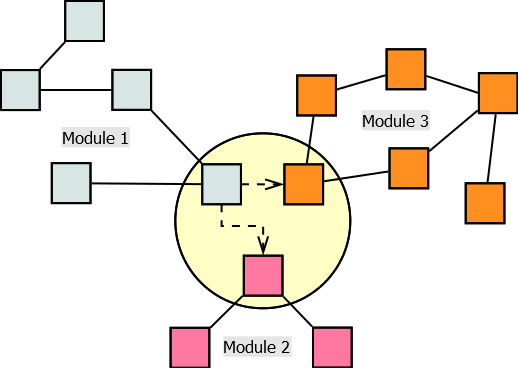
\includegraphics[width=0.48\textwidth]{Figures/Guice_modules.png}
  \end{center}
  \caption{Σύνθεση module μέσω της Guice}
  \label{fig:Guice}
\end{wrapfigure}

Στην υλοποίηση της βιβλιοθήκης χρησιμοποιήθηκε η Guice, ένα ελαφρύ 
πλαίσιο που υλοποιεί το πρότυπο dependency injection για την Java 
κατασκευασμένο από την Google. Όλες οι πληροφορίες παραμετροποίησης των 
συνδέσεων μεταξύ διεπαφών και υλοποιήσεων περιέχονται κυρίως σε ένα 
Module. Γενικά μια εφαρμογή που ακολουθεί αυτό το πρότυπο αποτελείται 
από διάφορα module και κώδικα που αφορά την αρχικοποίηση της.

Η κλάση που είναι υπεύθυνη για την κατασκευή των αντικειμένων είναι ο 
Injector. Για την αρχικοποίηση του χρειάζονται τα module. Σε γενικές 
γραμμές, όταν ζητηθεί η κατασκευή ενός αντικειμένου ενός τύπου, αρχικά 
βρίσκει τι να κατασκευάσει αφού μπορεί να υπάρχουν πολλές υλοποιήσεις. 
Στη συνέχεια λύνει τις εξαρτήσεις και αρχικοποιεί το αντικείμενο.

Κατά την εκκίνηση του συστήματος, όλη η παραμετροποίηση του όσον αφορά 
τι υλοποιήσεις θα χρησιμοποιηθούν παρέχεται από τα module όπως 
περιγράφηκε. Επιπλέον, έχουμε τη δυνατότητα αλλαγών κατά τη διάρκεια 
εκτέλεσης (runtime) του προγράμματος.

Ένα άλλο σημαντικό ζήτημα είναι και ο κύκλος ζωής των αντικειμένων που 
παράγονται. Αυτός ελέγχεται από τα λεγόμενα Scope. Αυτά περιγράφουν πόσο 
θα ζήσει ένα αντικείμενο κι αν είναι σε θέση να επαναχρησιμοποιηθεί. Οι 
λόγοι είναι επειδή είτε κρατάνε κατάσταση, είτε είναι ακριβά στην 
κατασκευή ή στη διατήρηση τους. Στην Guice προσφέρονται κάποια έτοιμα, 
τα οποία φαίνονται παρακάτω, αλλά παρέχεται και όλο το πλαίσιο να 
υλοποιηθούν νέα με την απαραίτητη λειτουργικότητα.

\newcounter{numberedCntE}
\begin{enumerate}
\item Unscoped: Το αντικείμενο παράγεται εκ νέου μετά από κάθε αίτηση 
κατασκευής στον injector.
\item Singleton: Το αντικείμενο που επιστρέφει ο injector είναι το ίδιο 
για όλη την εφαρμογή.
\item RequestScoped: Το αντικείμενο διαρκεί για μια web/rpc αίτηση 
(αφορά web εφαρμογές και servlet).
\item SessionScoped: Το αντικείμενο διαρκεί για μια HTTP συνεδρία. 
(αφορά web εφαρμογές και servlet).
\setcounter{numberedCntE}{\theenumi}
\end{enumerate}

\section{Δομή Υπηρεσίας}

Πλέον έχουμε την κατάλληλη βάση για την περιγραφή της δομής της 
υπηρεσίας που εισάγει η παρούσα αρχιτεκτονική. Οι αρχές που διέπουν τις 
υπηρεσίες και αναφέρθηκαν στην περιγραφή των υπηρεσιοκεντρικών 
συστημάτων είναι σημαντικό να εφαρμοστούν και στην παρούσα 
αρχιτεκτονική. Είναι απαραίτητο να υπάρχει μια ενιαία δομή αφού αυτό 
επιβάλλει μια ομοιομορφία στο επίπεδο. Το αποτέλεσμα είναι οι διάφορες 
υπηρεσίες να είναι εύκολα κατανοητές και το πιο σημαντικό είναι η 
ανάπτυξη ενός πλάνου για την υλοποίηση ή την τροποποίηση αυτών. Στο σχήμα 
\ref{fig:ServiceStructure} φαίνεται η δομή και ακολουθεί η εξήγηση καθώς και η 
αιτιολόγηση της ύπαρξής των στοιχείων από τα οποία αποτελείται. 

Να σημειωθεί πως για την κλήση απομακρυσμένων συναρτήσεων έχει 
χρησιμοποιηθεί η CORBA και προσθέτοντας κάποιες απαιτήσεις όσον αφορά 
την δομή της υπηρεσίας. Αυτό δε μας περιορίζει στο να αντικατασταθεί με 
κάποια άλλη βιβλιοθήκη. Οι αλλαγές που θα προκύψουν θα έχουν να κάνουν 
μόνο με τις διεπαφές και τις κλάσεις της CORBA.

\begin{figure}[htbp]
  \begin{center}
    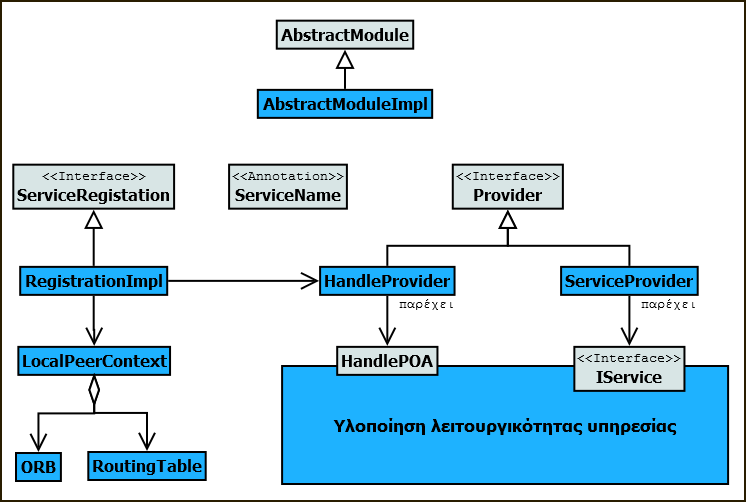
\includegraphics[width=0.95\textwidth]{Figures/Architecture/General_service_structure.png}
  \end{center}
  \caption{Γενική δομή υπηρεσίας}
  \label{fig:ServiceStructure}
\end{figure}

\paragraph{Διεπαφή Υπηρεσίας.} Όπως αναφέρθηκε στην ανάλυση των 
SOA συστημάτων, η υπηρεσία προσφέρει πρόσβαση στον χρήστη σε μια ή 
περισσότερες λειτουργίες. Είναι φυσικό να υπάρχει η διεπαφή που καθορίζει 
τις ενέργειες που μπορούν να γίνουν. Μέσω αυτής της διεπαφής πρέπει να 
περιγράφεται όλο εκείνο το πλαίσιο στο οποίο εκτελείται η υπηρεσία 
εννοώντας τους περιορισμούς που τίθενται. Η διεπαφή IService του σχήματος 
\ref{fig:ServiceStructure} αντιπροσωπεύει μια τέτοια διεπαφή. Γύρω από αυτήν 
μπορεί να υπάρξουν και άλλες βοηθητικές κλάσεις ή διεπαφές. Για παράδειγμα 
είναι πιθανό κατά την εκτέλεση μιας υπηρεσίας να αλλάξει μονοπάτι ο peer. 
Αυτή η πληροφορία μπορεί να αφορά άμεσα την εφαρμογή και θα πρέπει ως 
αποτέλεσμα να υπάρξει συγκεκριμένη αντίδραση. Το πρόβλημα αυτό λύνεται 
με το σχεδιαστικό πρότυπο Observer \citep{GoF} ή Listener όπως ονομάζεται 
αλλιώς στον κόσμο της Java.

\paragraph{Java IDL (Servant).} Η δυνατότητα εκτέλεσης της υπηρεσίας ως 
απομακρυσμένης κλήσης συνάρτησης (rpc) ικανοποιείται από την CORBA. Κατ' 
επέκταση είναι αναγκαία η περιγραφή της υπηρεσίας σε IDL. Από αυτήν 
παράγονται οι απαραίτητοι τύποι. Ανάμεσα σε αυτούς είναι και ο Servant 
%$[$παραπομπή$]$ 
ο οποίος παρέχει την ίδια λειτουργικότητα με την 
υπηρεσία. Είναι εκείνο το αντικείμενο που θα κληθεί όταν ένας peer λάβει 
μια αίτηση εκτέλεσης της υπηρεσίας.

\paragraph{Διεπαφή Provider.} Η κατασκευή αντικειμένων των υλοποιήσεων είτε 
της υπηρεσίας είτε του Servant μπορεί να είναι μια πολύπλοκη διαδικασία 
η οποία δε θα έπρεπε να απασχολεί τον χρήστη. Στην προκειμένη περίπτωση, 
η Guice έχει αναλάβει την κατασκευή τους. Οι κλάσεις που υλοποιούν την 
διεπαφή Provider είναι ικανές να παρέχουν συγκεκριμένα αντικείμενα. 
Περιγράφουν στην Guice τον τρόπο με τον οποίο κατασκευάζονται πολύπλοκοι 
τύποι. Επίσης, μέσω των Provider μπορούμε να ελέγξουμε τον κύκλο ζωής 
τον αντικειμένων που επιστρέφει. Παράδειγμα η υλοποίηση του Servant δεν 
έχει νόημα να κατασκευάζεται συνεχώς εκ νέου. Έχει επιλεχθεί επομένως ο 
Provider του να συμπεριφέρεται ως singleton και έτσι να επιστρέφει το 
ίδιο αντικείμενο όταν του ζητείται. Σε αντίθεση με την υλοποίηση της 
διεπαφής της υπηρεσίας όπου εκεί μπορούμε να κατασκευάζουμε νέο κάθε 
φορά. Βέβαια υπάρχουν και περιπτώσεις όπου, όπως περιγράφηκε στην 
ενότητα του Dependency Injection, μπορεί να είναι ακριβό η συνεχής 
κατασκευή.

\paragraph{Εγκατάσταση υπηρεσίας.} Τον χρήστη της υπηρεσίας δεν τον 
απασχολεί ο τρόπος με τον οποίο ένας peer ξεκινά να εξυπηρετεί 
απομακρυσμένες αιτήσεις μιας υπηρεσίας. Αυτό καλύπτεται από την διεπαφή 
ServiceRegistration. Στην παρούσα φάση όπου εξαρτόμαστε από την CORBA, 
τα βήματα είναι η δημιουργία ενός Servant της υπηρεσίας που θέλουμε και 
η εγκατάστασή του στον POA. Για να επιτευχθεί αυτό χρειάζεται μια 
αναφορά προς το ORB του peer. Αυτή μπορεί να ληφθεί μέσω του 
LocalPeerContext που κρατά πληροφορίες για τον τοπικό peer, αναφορές 
προς τον πίνακα δρομολόγησης του και το ORB του.

Η διεπαφή ServiceRegistration πρόκειται να έχει τόσες υλοποιήσεις όσες 
και οι υπηρεσίες του συστήματος. Είναι αναγκαίος ένας τρόπος ώστε η 
Guice να ξέρει ποια να επιστρέφει όταν ζητείται μιας συγκεκριμένης 
υπηρεσίας. Αυτό επιτυγχάνεται με τη δημιουργία ενός annotation. Στην 
εικόνα \ref{fig:ServiceStructure} το ServiceName παίζει αυτόν τον ρόλο.

\paragraph{Λειτουργικότητα Υπηρεσίας.} Μετά τον καθορισμό των παραπάνω 
έχουμε την υλοποίηση της υπηρεσίας όπου προσφέρεται η λειτουργικότητά της. 
Εδώ έχουμε τον χώρο για την δήλωση όλων των βοηθητικών διεπαφών και κλάσεων 
καθώς και των υλοποιήσεών του. Είναι προφανές πως η λογική που θα 
ακολουθηθεί εδώ κρίνει και κατά πόσο η υπηρεσία θα καταστεί επεκτάσιμη 
και τροποποιήσιμη. Στην εικόνα \ref{fig:ServiceStructure} φαίνεται αυτό 
το κομμάτι καθώς και οι διεπαφές που το καλύπτουν.

\paragraph{Παραμετροποίηση Module.} Τελικά, καταλήγουμε να έχουμε υλοποιήσεις όλων 
των αναγκαίων κλάσεων και διεπαφών καθώς και εκείνου του κομματιού που 
έχει σχέση με την αυτή καθεαυτή λειτουργικότητα της υπηρεσίας. Αυτό που 
απομένει είναι η δήλωση όλων των αντιστοιχίσεων διεπαφών/κλάσεων με τις 
υλοποιήσεις τους ώστε να γνωρίζει η Guice τον τρόπο με τον οποίο θα 
παράγει αντικείμενα αυτών λύνοντας τις εξαρτήσεις τους. Η υλοποίηση της 
κλάσης AbstractModule που προσφέρεται από την Guice εξυπηρετεί αυτόν τον 
σκοπό. Να σημειωθεί πως μπορεί να έχουμε αρκετές υλοποιήσεις της ίδιας 
υπηρεσίας. Κατά την εκκίνηση του προγράμματος θα έχουμε μια συσχέτιση με 
συγκεκριμένη υλοποίηση. Παρόλα αυτά μπορεί να είναι αναγκαίο κατά τον 
χρόνο εκτέλεσης του συστήματος να γίνει αλλαγή σε άλλη υλοποίηση της 
υπηρεσίας. Η συμπεριφορά αυτή δηλώνεται στο Module ως multibindings όσον 
αφορά τον τρόπο με τον οποίο το επιτυγχάνει η Guice.

\section{Δομή Διαδικασιών}

\begin{figure}[htbp]
  \begin{center}
    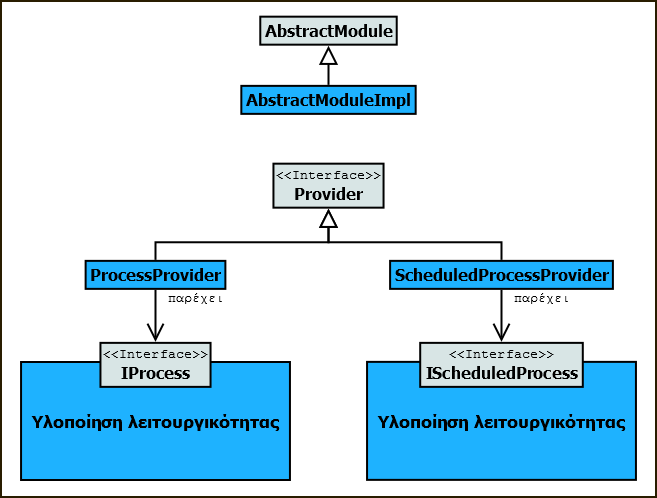
\includegraphics[width=0.95\textwidth]{Figures/Architecture/General_process_structure.png}
  \end{center}
  \caption{Γενική δομή διαδικασίας}
  \label{fig:ProcessStructure}
\end{figure}

Όπως αναφέρθηκε η διαδικασία είναι αποτέλεσμα της σύνθεσης 
διάφορων υπηρεσιών. Στόχος είναι να παραχθεί λειτουργικότητα που έχει 
νόημα και είναι χρήσιμη στην εφαρμογή. Στην ουσία η διαδικασία είναι και 
αυτή ένας τύπος υπηρεσίας.Εδώ υπάρχει μεγαλύτερη ελευθερία αφού 
εδώ η γενική δομή που απεικονίζεται στο σχήμα \ref{fig:ProcessStructure} 
είναι απλά ενδεικτική.

\paragraph{Διεπαφή διαδικασίας.} Η περιγραφή της λειτουργικότητας και των 
περιορισμών που θέτει η διαδικασία γίνεται μέσω της διεπαφής της.

\paragraph{Provider.} Όπως και στις υπηρεσίες, έτσι κι εδώ, μια διαδικασία 
μπορεί να είναι πολύπλοκη στην κατασκευή. Ένας Provider αναλαμβάνει να 
κατασκευάσει τέτοια αντικείμενα αποκρύπτοντας τον τρόπο από τον χρήστη.

\paragraph{Παραμετροποίηση Module.} Αντίστοιχα, οι αντιστοιχίσεις 
διεπαφών/κλάσεων με τις υλοποιήσεις τους που αφορούν την Guice 
βρίσκονται στο Module της διαδικασίας.

Πέρα από την απλή σύνθεση των διαδικασιών, μπορούν να εισαχθούν 
νέες έννοιες (semantics). Στην παρούσα φάση, πέρα από την απλή, έχουμε 
την έννοια της προγραμματιζόμενης διαδικασίας. Για να γίνει μια 
διαδικασία προγραμματισμένη ώστε να εκτελείται ανά τακτά χρονικά 
διαστήματα, πρέπει να υλοποιηθεί η κλάση TimerTask της Java. Όσον αφορά 
την Guice, για τον διαχωρισμό τον υλοποιήσεων, χρειάζεται η ανάγκη ενός 
annotation που να δηλώνει την παραπάνω έννοια.

\chapter{Πρωτόκολλα Αρχιτεκτονικής}
\label{chap:Protocols}

\section{Εισαγωγή}

Στο παρόν κεφάλαιο περιγράφονται τα πρωτόκολλα του συστήματος. Η βιβλιοθήκη 
έχει βασιστεί στο P-Grid και επομένως υλοποιείται ο αλγόριθμος exchange 
όπως έχει οριστεί στο \citep{Abererb}. Θα γίνει μια μικρή περιγραφή του. 
Στη συνέχεια αναλύεται διεξοδικά το πρωτόκολλο ανοχής λαθών που η ανάπτυξή 
του είναι και ένας από τους στόχους της διπλωματικής εργασίας.

\section{Πρωτόκολλο Exchange}

To P-Grid δίκτυο κατασκευάζεται μέσω των αλληλεπιδράσεων μεταξύ των peer. 
Ο τρόπος με τον οποίο ένα P-Grid δίκτυο κατασκευάζεται είναι μέσω του 
αλγορίθμου exchange. Στα σχήματα \ref{algo:ExchangePart1} και 
\ref{algo:ExchangePart2} παρουσιάζεται ο αλγόριθμος και ακολουθεί η 
ανάλυση του.

Αρχικά, κατά τα πρώτα στάδια εκκίνησης του δικτύου, οι peer είναι υπεύθυνοι 
για όλο τον χώρο κλειδιών. Δεν υπάρχουν κατατμίσεις και όλοι οι peer 
αντιστοιχούν στο ριζικό μονοπάτι του δέντρου. Ο αλγόριθμος exchange 
καθορίζει τον τρόπο με τον οποίο ο χώρος κλειδιών θα διασπαστεί σε 
περισσότερες εξειδικεύσεις. Κάθε μια από αυτές τίθεται υπό την ευθύνη 
ενός peer. Ο αλγόριθμος εκτελείται με την πρώτη ευκαιρία που δύο peer 
θα συναντηθούν.

Οι peer ελέγχονται πάνω στο μονοπάτι για το οποίο είναι υπεύθυνοι. 
Σε κάθε εκτέλεση του αλγορίθμου, οι δυο peer ανανεώνουν τους πίνακες 
δρομολόγησης τους. Αρχικά, ανταλλάσουν τυχαία αναφορές προς peer για όλα τα 
επίπεδα του κοινού προθέματος.

\paragraph{Περίπτωση 1.} Η πρώτη περίπτωση του αλγορίθμου προκύπτει όταν 
αυτοί αντιστοιχούν στο ίδιο μονοπάτι, έστω $x$. Τότε και οι δύο peer 
εξειδικεύονται περαιτέρω προς αντίθετες κατευθύνσεις. Ο ένας θα αναλάβει 
το μονοπάτι $χ0$ και ο άλλος το συζυγές $χ1$. Κάθε peer προσθέτει τον άλλον 
στον πίνακα δρομολόγησης ως υπεύθυνο για το νέο επίπεδο που προστέθηκε στο 
μονοπάτι.

\paragraph{Περιπτώσεις 1 και 2.}Η δεύτερη και η τρίτη περίπτωση είναι 
παρόμοιες. Το μονοπάτι του ενός peer είναι μικρότερο από αυτό του άλλου 
και μάλιστα είναι και πρόθεμα του. Στην περίπτωση αυτή, ο λιγότερο 
εξειδικευμένος peer προχωρά προς την αντίθετη κατεύθυνση. Αν παράδειγμα 
αυτός είχε το μονοπάτι $x$ και ο άλλος peer το $χ1$, τότε εξειδικεύεται 
προς το $x0$. Επίσης, ανανεώνονται και οι αναφορές στους πίνακες 
δρομολόγησης. Παρατειρούμε, πως αν ο peer $a1$ αντιστοιχεί το μικρότερο 
μονοπάτι, τότε κατά την εκτέλεση του αλγορίθμου αυτός θα είναι στην 
δεύτερη περίπτωση ενώ ο $a2$ στην τρίτη.

\paragraph{Περίπτωση 4.} Τέλος, έχουμε την περίπτωση όπου οι δυο peer 
μοιράζονται ένα κοινό πρόθεμα αλλά από εκεί και μετά έχουν ακολουθήσει 
διαφορετικού δρόμους στο δέντρο. Εδώ ο αλγόριθμος εκτελείται αναδρομικά. 
Οι peer $a1$ και $a2$ προωθούν αιτήσεις για εκτέλεση του αλγορίθμου στους 
peer που έχουν αποθηκευμένους στους πίνακες δρομολόγησης. Όταν 
το δίκτυο φτάσει στην τελική του μορφή, ο χώρος κλειδιών θα έχει διασπαστεί 
σε τόσα κομμάτια όσα και ο αριθμός των peer. Τότε θα προκύπτει συνεχώς η 
τέταρτη περίπτωση κατά την εκτέλεση του αλγορίθμου. Η σταθερά $recmax$ 
θέτει ένα άνω όριο στον αριθμό των αναδρομών που θα εκτελεστούν και είναι 
μια συνθήκη τερματισμού.

%Στην αρχική μορφή του αλγορίθμου που περιγράφεται στη δημοσίευση 
%\citep{Abererb}, τίθεται ένα όριο μέχρι το οποίο μπορεί να εξειδικευτούν 
%οι peer. Ο λόγος ήταν η ομοιόμορφη κατανομή των μονοπατιών θεωρώντας πως 
%επηρεάζει

\begin{algorithm}
\caption{Αλγόριθμος exchange, μέρος 1ο}
\label{algo:ExchangePart1}
\begin{algorithmic}[1]
    \Procedure{exchange}{a1, a2, r} 
        \State commonpath = common\_prefix\_of(path(a1), path(a2));
        \State lc = length(commonpath);
        \If{(lc > 0)}
        \Comment{exchange references at the level where the paths agree}
            \State commonrefs = union(refs(lc, a1), refs(lc, a2));
            \State refs(lc, a1) = random\_select(refmax, commonrefs);
            \State refs(lc, a2) = random\_select(refmax, commonrefs);
            \State l1 = length(sub\_path(path(a1), lc + 1, length(path(a1))));
            \State l2 = length(sub\_path(path(a2), lc + 1, length(path(a2))));            
\newline \Comment{Case 1: if both remaining paths are empty introduce a new level}
            \If{(l1 = 0 $\And$ l2 = 0)}            
                \State path(a1) = append(path(a1), 0);
                \State path(a2) = append(path(a2), 1);
                \State refs(lc + 1, a1) = {a2};
                \State refs(lc + 1, a2) = {a1};
            \EndIf
\newline \Comment{Case 2: if one remaining path is empty split the shorter path}
            \If{(l1 = 0 $\And$ l2 > 0)}
                \State path(a1) = append(path(a1), $\neg$value(lc + 1, path(a2)));
                \State refs(lc + 1, a1) = {a2};
                \State refs(lc + 1, a2) = random\_select(refmax, union({a1}, refs(lc + 1, a2)));
            \EndIf
\algstore{ExchangeBreak}
\end{algorithmic}
\end{algorithm}

\begin{algorithm}[h]
\caption{Αλγόριθμος exchange, μέρος 2ο}
\label{algo:ExchangePart2}
\begin{algorithmic}[1]
\algrestore{ExchangeBreak}
\item[] \Comment{Case 3: like case 2}
            \If{(l1 > 0 $\And$ l2 = 0)}
                \State path(a2) = append(path(a2), $\neg$value(lc + 1, path(a1)));
                \State refs(lc + 1, a2) = {a1};
                \State refs(lc + 1, a1) = random\_select(refmax, union({a2}, refs(lc + 1, a1)));
            \EndIf
\newline \Comment{Case 4: recursively perform exchange with referenced peers}
            \If{(l1 > 0 $\And$ l2 > 0 $\And$ r < recmax)}
                \State refs1 = refs(lc + 1, a1) $\setminus$ {a2};
                \State refs2 = refs(lc + 1, a2) $\setminus$ {a1};
                \For{r1 $\in$ refs1}
                    \If{online(peer(r1))}
                        \State exchange(a2, peer(r1), r + 1)
                    \EndIf
                \EndFor
                \For{r2 $\in$ refs2}
                    \If{online(peer(r2))}
                        \State exchange(a1, peer(r2), r + 1)
                    \EndIf
                \EndFor
            \EndIf
        \EndIf
  \EndProcedure
\end{algorithmic}
\end{algorithm}


\section{Πρωτόκολλο Ανοχής Λαθών (Fault-Tolerance)}

\ \ \ \ TODO

\chapter{Υλοποίηση Αρχιτεκτονικής}
\label{chap:Impl}

\section{Εισαγωγή}

Η υλοποίηση της προτεινόμενης αρχιτεκτονικής έγινε με τη χρήση 
της γλώσσας προγραμματισμού Java. Όπως έχει αναφερθεί η Guice 
χρησιμοποιήθηκε για την υποστήριξη του προτύπου dependency injection. Η 
υλοποίηση της CORBA που προσφέρεται από την Java καλύπτει τις ανάγκες 
απομακρυσμένων κλήσεων συναρτήσεων. Η ανάγκη καταγραφής μηνυμάτων 
καλύφθηκε από την βιβλιοθήκη log4j και της slf4j. Τέλος, για την 
διενέργεια ελέγχων χρησιμοποιήθηκε η βιβλιοθήκη JUnit.

Έγινε χρήση διάφορων εργαλείων όπως το Ant το οποίο καθοδηγεί 
μεταγλώττιση, την εκτέλεση των unit test, την εξαγωγή της τεκμηρίωσης 
μέσω javadoc και την δημιουργία της βιβλιοθήκης ως jar αρχείου. Αναγκαία 
ήταν διάφορα εργαλεία στατικής ανάλυσης του κώδικα που προσφέρονταν μέσω 
του IDE IntelijIDEA. Για την διαχείριση του κώδικα και των εκδόσεων του 
χρησιμοποιήθηκε το git. Ο κώδικας της βιβλιοθήκης υπάρχει στο αποθετήριο 
\url{https://github.com/Archimidis/pgrid}

\section{Common Object Request Broker Architecture (CORBA)}

Η υλοποίηση βασίστηκε πάνω στην CORBA 
\citep{CorbaSpec, CorbaSpecP1, CorbaSpecP2, CorbaSpecP3} για 
την επικοινωνία των peer μέσω κλήσεων απομακρυσμένων συναρτήσεων (rpc). 
Η δομή της αρχιτεκτονικής της δε μας αφορά. Είναι σημαντικές, όμως, 
κάποιες λεπτομέρειες οι οποίες αφορούν την περαιτέρω παραμετροποίηση του 
συστήματος. 

Για την υλοποίηση των υπηρεσιών πρέπει να γραφεί σε idl η περιγραφή 
αυτής. Μέσω της idl παράγονται ο κώδικας που είναι χρήσιμος για την 
κλήση μιας συνάρτησης client (stub code) και ο κώδικας για την 
εξυπηρέτηση αυτών των κλήσεων (skeleton code). Το δεύτερο κομμάτι είναι 
εκεί όπου υλοποιείται η λειτουργικότητα της διεπαφής. Η προώθηση των 
κλήσεων σε αυτό γίνεται μέσω του servant.

Ένα σημαντικό κομμάτι της αρχιτεκτονικής που ενδιαφέρει και εμάς είναι ο 
Portable Object Adapter (POA). Ο ρόλος του είναι να ενώσει τους servant 
με το ORB και η διαχείριση του περιβάλλοντος το αντικείμενο που είναι η 
υλοποίηση της διεπαφής κατά τον χρόνο εκτέλεσης. Μέσω αυτού γίνεται η 
αντιστοίχιση servant με υλοποιήσεις. Επίσης, ο POA μπορεί να 
ενεργοποιήσει το αντικείμενο και η προσαρμογή του σε συγκεκριμένες 
πολιτικές. Το τελευταίο είναι που προσθέτει επιπλέον δυνατότητες 
παραμετροποίησης του συστήματος.

Οι πολιτικές που χρησιμοποιούνται από τον POA είναι οι παρακάτω 
\citep{CorbaProg2001}:

\newcounter{numberedCntBC}
\begin{enumerate}
\item \textbf{Μοναδικότητα ID.} Καθορίζει αν περισσότερα από ένα ID 
αντικειμένου θα αναφέρεται στον ίδιο servant.
\item \textbf{Ανάθεση ID.} Καθορίζει αν την ανάθεση των ID την κάνει ο 
POA ή ο προγραμματιστής.
\item \textbf{Διάρκεια ζωής.} Καθορίζει αν τα αντικείμενα είναι 
παροδικά ή μόνιμα. Αν το αντικείμενο, δηλαδή, είναι προσιτό μετά την 
καταστροφή του POA ή όχι.
\item \textbf{Διατήρηση servant.} Καθορίζει αν ο POA κρατά τις 
συσχετίσεις μεταξύ ID αντικειμένου και servant σε μια δομή που 
ονομάζεται Active Object Map. Σε αντίθετη περίπτωση στηρίζεται στον 
προεπιλεγμένο servant ή σε servant locator για τον εντοπισμό του 
κατάλληλου servant με στόχο την εξυπηρέτηση της αίτησης.
\item \textbf{Επεξεργασία αίτησης.} Καθορίζει αν ο POA χρησιμοποιεί 
είτε μόνο το Active Object Map, είτε μόνο τον προεπιλεγμένο servant είτε 
την χρήση του servant manager. Η επιλογή που θα γίνει για την διατήρηση 
του servant επηρεάζει και τον τρόπο με τον οποίο θα γίνει η επεξεργασία. 
Συγκεκριμένα για τον servant manager υπάρχουν δυο κατηγορίες
\begin{itemize}
\item \textbf{Servant activator.} βάσει αυτού δημιουργείται ο servant 
και όταν τελειώσει ο κύκλος ζωής του τότε καταστρέφεται.
\item \textbf{Servant locator.} Εύρεση του κατάλληλου servant ο οποίος 
δεν είναι καταχωρημένος στο Active Object Map.
\end{itemize}
\item \textbf{Πολιτική νημάτων.} Καθορίζει αν θα ακολουθηθεί 
μονονηματική πολιτική ή όχι.
\item \textbf{Σιωπηρή ενεργοποίηση servant.} Καθορίζει αν ο POA μπορεί 
να ενεργοποιήσει έναν servant όταν μια αναφορά προς ένα ID δημιουργηθεί.
\setcounter{numberedCntBC}{\theenumi}
\end{enumerate}
Μπορούν συνδυασμοί μπορούν να προκύψουν από τα παραπάνω. Η χρήση μόνο 
του Active Object Map για την επεξεργασία των αιτήσεων συνοδεύεται με 
την επιλογή της αποθήκευσης αντιστοιχίσεων ID και servant σε αυτόν. 
Πρέπει να γνωρίζουμε πριν την εκκίνηση του συστήματος τον αριθμό των 
servant αφού αυτοί θα δημιουργηθούν και θα εγκατασταθούν ρητά.

Στην περίπτωση που ο αριθμός των αντικειμένων είναι μεγάλος ή δεν τον 
γνωρίζουμε εξ αρχής τότε είναι χρήσιμος ο servant manager. Αν επιλέξουμε 
την ύπαρξη αντιστοιχίσεων στο Active Object Map, τότε χρησιμοποιείται ο 
servant activator. Αν δεν βρεθεί ένα αντικείμενο μέσω του ID του τότε 
ενεργοποιείται ο κατάλληλος servant. Σε αντίθετη περίπτωση όπου δεν 
έχουμε Active Object Map τότε χρησιμοποιείται ο servant locator. Ο 
servant επιτρέπει την παροχή διαφορετικών servant που αντιστοιχούν σε 
διαφορετικές υλοποιήσεις της διεπαφής που καλείται.

Συνεπώς, παρέχοντας υλοποιήσεις των servant manager μπορούμε να 
καθορίσουμε περαιτέρω τον κύκλο ζωής των υπηρεσιών και των αντικειμένων 
που χρησιμοποιούν ανάλογα με τις απαιτήσεις του περιβάλλοντος στο οποίο 
εκτελείται ο peer.

\section{Επίπεδο Οντοτήτων - Entity Layer}

Όπως έχει αναφερθεί στο επίπεδο οντοτήτων υπάρχει οτιδήποτε 
αποθηκεύει κατάσταση ή δεδομένα και παρέχει πρόσβαση σε υπηρεσίες που 
προσφέρει το λειτουργικό σύστημα πάνω στο οποίο εκτελείται η εφαρμογή.

Ένας peer για να περιγραφεί ολοκληρωμένα χρειάζεται η διεύθυνσή 
του (ip και port). Επίσης, μετά την εισαγωγή του στο δίκτυο είναι 
υπεύθυνος για ένα κομμάτι του χώρου κλειδιών το οποίο καθορίζεται από το 
μονοπάτι που του έχει δοθεί. Χρειάζεται και αυτή η πληροφορία. Τέλος, 
κάθε peer αναγνωρίζεται μοναδικά από ένα UUID που του δίνεται κατά την 
εκκίνησή του. Τα παραπάνω περιγράφονται από την διεπαφή Host.

Δίνονται διεπαφές που αναπαριστούν ένα κλειδί, Key, καθώς και ενός 
πεδίου κλειδιών, KeyRange, του συστήματος. Τα κλειδιά όπως έχει 
αναφερθεί συσχετίζονται είτε με peer είτε με πόρους που προσφέρονται από 
τους peer στο δίκτυο. Επίσης, προσφέρεται διεπαφή που αφορά τα μονοπάτια 
του P-Grid δέντρου, PGridPath. Διαφορετική σημασιολογία ή αναπαράσταση 
σε όλα τα παραπάνω μπορεί να δοθεί επεκτείνοντας αυτές τις διεπαφές. Η 
παραγωγή αντικειμένων αυτών των τύπων για χρήση από τον χρήστη γίνεται 
μέσω του σχεδιαστικού προτύπου factory \citep{GoF}.

Η έννοια του χρόνου σε ένα κατανεμημένο σύστημα είναι σημαντική για την 
σειριοποίηση των γεγονότων που συμβαίνουν σε αυτό. Υπάρχει η έννοια του 
ρολογιού στην διεπαφή PeerClock και δίνεται επίσης η κλασική υλοποίηση 
των Lamport ρολογιών \citep{Lamport}. Η υλοποίηση είναι ασφαλής για σε 
πολυνηματικό κώδικα.

Κάθε peer που μετέχει στο δίκτυο αποθηκεύει αναφορές προς άλλους 
peer. Ο τρόπος και η δομή με την οποία αποθηκεύονται αυτές εκφράζονται 
μέσω του πίνακα δρομολόγησης, RoutingTable. Η παραγωγή αντικειμένων 
αυτού του τύπου επιτυγχάνεται με τη χρήση του σχεδιαστικού προτύπου 
abstract factory \citep{GoF}. Η υλοποίηση που παρέχεται για τον 
πίνακα δρομολόγησης είναι ασφαλής για χρήση σε πολυνηματικό κώδικα, 
δεδομένης της ταυτόχρονης χρήσης από πολλές υπηρεσίες.

Η επικοινωνία μεταξύ των peer του δικτύου επιτυγχάνεται μέσω 
απομακρυσμένων κλήσεων συναρτήσεων (rpc). Αυτή η 
λειτουργικότητα προσφέρεται από την CORBA. Ως οντότητα θεωρείται το ORB 
και επιπλέον για την ρύθμισή του και την παραγωγή του κατά την εκκίνηση 
του peer χρησιμοποιείται abstract factory. Κάθε ORB είναι μοναδικό για 
κάθε peer και πρέπει να υπάρχει ένα αντικείμενο αυτού του τύπου ανά 
εφαρμογή.

Στην \ref{fig:EntityLayer} φαίνεται το UML διάγραμμα κλάσεων που αφορά 
το επίπεδο οντοτήτων. Η κλάση EntityModyle περιέχει την παραμετροποίηση 
που απαιτείται από την Guice.

\begin{figure}[htbp]
  \begin{center}
    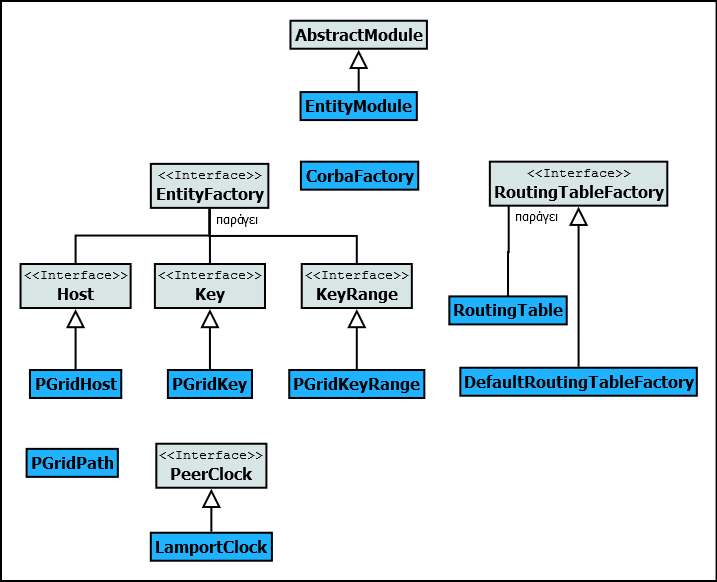
\includegraphics[width=0.9\textwidth]{Figures/Architecture/Entity_Layer/EntityLayer_ClassDiagram.png}
  \end{center}
  \caption{Διάγραμμα κλάσεων επιπέδου οντοτήτων}
  \label{fig:EntityLayer}
\end{figure}

\section{Επίπεδο Υπηρεσιών - Service Layer}

Στο επίπεδο των υπηρεσιών υπάρχουν όλα τα πρωτόκολλα που 
προσφέρει το σύστημα εκφρασμένα ως υπηρεσίες. Στην παρούσα φάση της 
υλοποίησης έχουμε το πρωτόκολλο Exchange και αυτό της ανοχής λαθών 
Repair, όπως αυτά έχουν περιγραφεί. Επίσης, έχει υλοποιηθεί μια υπηρεσία 
που αφορά την προσομοίωση του συστήματος και βοηθά στον έλεγχό του. Στις 
επόμενες ενότητες θα αναλυθούν οι υλοποιήσεις των προαναφερθέντων. 
Παρέχεται, επίσης και μια υπηρεσία για την αρχικοποίηση του συστήματος.

Στο διάγραμμα συστατικών (component) \ref{fig:ServiceComponents} 
φαίνονται οι μονάδες του επιπέδου. Το επίπεδο περιλαμβάνει τα module 
των υπηρεσιών Exchange, Repair, Simulation και αρχικοποίησης. Επίσης, 
φαίνονται οι τρεις διεπαφές που εκτίθενται στα ανώτερα επίπεδα καθώς και 
οι εξαρτήσεις του παρόντος από το επίπεδο οντοτήτων. Επίσης, κάθε υπηρεσία 
έχει ανάγκη το ORB για επικοινωνία και τον πίνακα δρομολόγησης του τοπικού 
peer. Αυτά αποθηκεύονται στην κλάση LocalPeerContext. Κάθε κατά την διάρκεια 
εκτέλεσης του συστήματος, υπάρχει μόνο αντικείμενο αυτής της κλάσης το 
οποίο επιστρέφεται από την Guice.

\begin{figure}[htbp]
  \begin{center}
    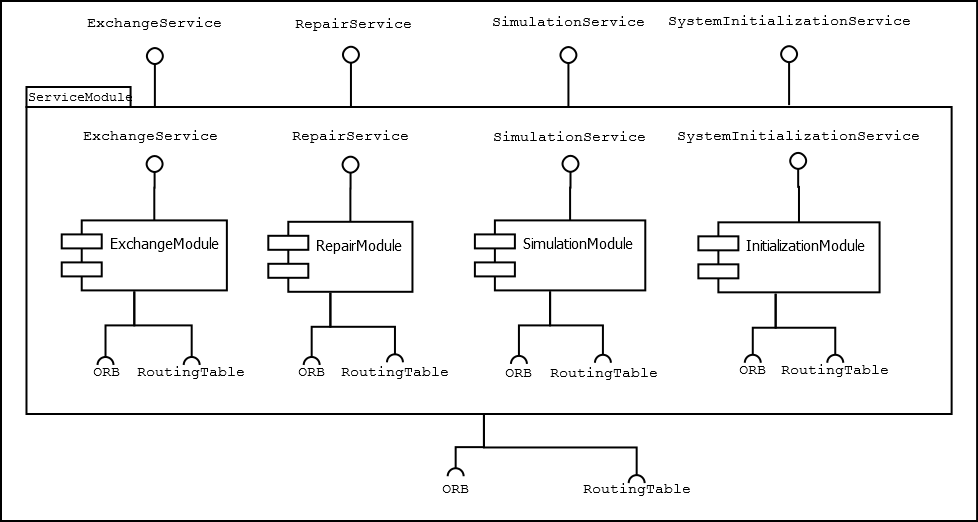
\includegraphics[width=0.9\textwidth]{Figures/Architecture/Service_Layer/Service_ComponentDiagram.png}
  \end{center}
  \caption{Διάγραμμα συστατικών επιπέδου υπηρεσιών}
  \label{fig:ServiceComponents}
\end{figure}

\subsection{Υλοποίηση Πρωτοκόλλου Exchange ως Υπηρεσία}

\begin{figure}[htbp]
  \begin{center}
    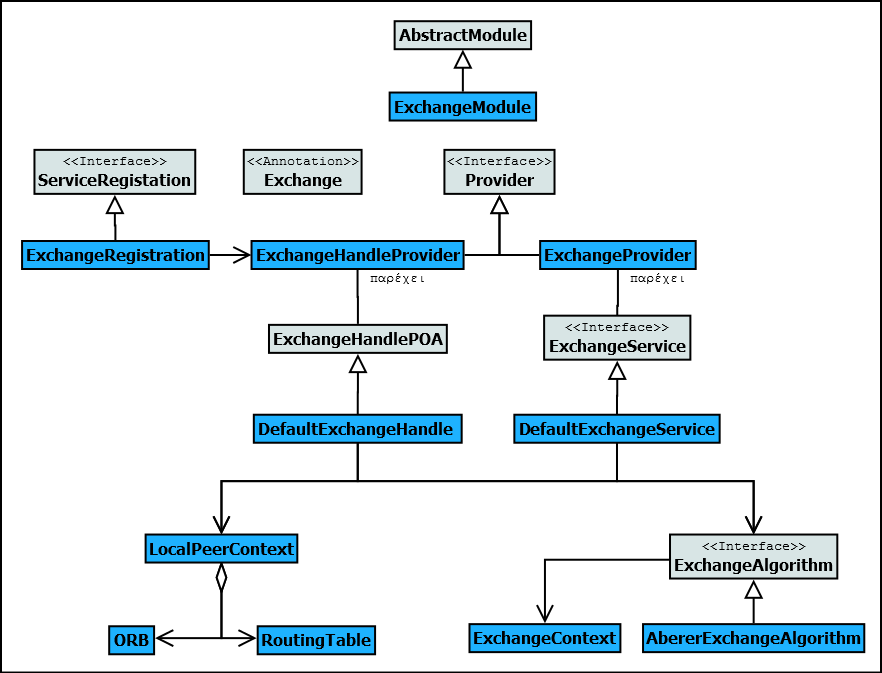
\includegraphics[width=0.9\textwidth]{Figures/Architecture/Service_Layer/ExchangeService_ClassDiagram.png}
  \end{center}
  \caption{Διάγραμμα κλάσεων υπηρεσίας Exchange}
  \label{fig:ExhangeService}
\end{figure}

Στην εικόνα \ref{fig:ExhangeService} φαίνεται το διάγραμμα κλάσεων της 
υπηρεσίας Exchange. Η δομή της ακολουθεί την γενική δομή της υπηρεσίας που 
περιγράφηκε σε προηγούμενη ενότητα. 

Η διεπαφή που εκθέτει την λειτουργικότητα της υπηρεσίας στο επίπεδο των 
διεργασιών και της εφαρμογή είναι η ExchangeService. Με την κλήση της 
μεθόδου που προσφέρει, ο τοπικός peer επικοινωνεί με τον απομακρυσμένο 
peer που έχει δοθεί ως όρισμα και εκτελούν τον αλγόριθμο exchange. Στην 
περίπτωση όπου υπάρχει πρόβλημα κατά την επικοινωνία, αν παράδειγμα ο 
απομακρυσμένος peer έχει αποτύχει, η υπηρεσία τερματίζει χωρίς να 
εκτελέσει τον αλγόριθμο με ένα CommunicationException.

Αντίστοιχα, για την πλευρά του εξυπηρετητή του peer που αφορά την CORBA 
έχουμε την κλάση ExchangeHandlePOA που έχει παραχθεί μέσω της idl. 
Παρέχει την υλοποίηση του CORBA αντικειμένου η οποία θα εγκατασταθεί 
στην CORBA και θα μπορεί να εξυπηρετεί απομακρυσμένες αιτήσεις εκτέλεσης 
του αλγορίθμου.

Οι παραπάνω διεπαφές έχουν μια προεπιλεγμένη υλοποίησης. Αυτές 
σχετίζονται με την διεπαφή ExchangeAlgorithm και της υλοποίησης της, την κλάση 
AbererExchangeAlgorithm. Η μέθοδος που προσφέρει δέχεται ένα αντικείμενο 
τύπου ExchangeContext. Το ExchangeContext περιέχει όλη την πληροφορία 
που χρειάζεται, όπως ο πίνακας δρομολόγησης, για να εκτελεστεί ο 
αλγόριθμος.

Για την κατασκευή αντικειμένων των τύπων που δηλώνονται από τις διεπαφές 
ExchangeService και ExchangeHandlePOA υλοποιείται η διεπαφή Provider. Ο 
ExchangeProvider παρέχει νέα αντικείμενα της ExchangeService σε κάθε 
αίτηση παροχής. 

Αρχικοποιεί την υπηρεσία με όλα τα απαραίτητα αντικείμενα και σταθερές 
όπως ο μέγιστος αριθμός αναδρομών που θα εκτελεστεί ο αλγόριθμος. 
Αντίστοιχα για την ExchangeHandlePOA έχουμε τον ExchangeHandleProvider, 
μόνο που εδώ παρέχεται πάντα το ίδιο αντικείμενο σε κάθε αίτηση.

Για την εγκατάσταση της υπηρεσίας στην CORBA έχουμε την υλοποίηση της 
διεπαφής ServiceRegistration, την ExchangeRegistration. Για να 
διευκρινιστεί στην Guice ποια υλοποίηση της ServiceRegistration θέλουμε, 
έχουμε το Annotation Simulation.

Τέλος, η όλη σύνδεση διεπαφών και υλοποιήσεων καθώς και τον καθορισμό 
του κύκλου ζωής των αντικειμένων βρίσκεται στην κλάση ExchangeModule.

\subsection{Υλοποίηση Πρωτοκόλλου Repair ως Υπηρεσία}

\begin{figure}[htbp]
  \begin{center}
    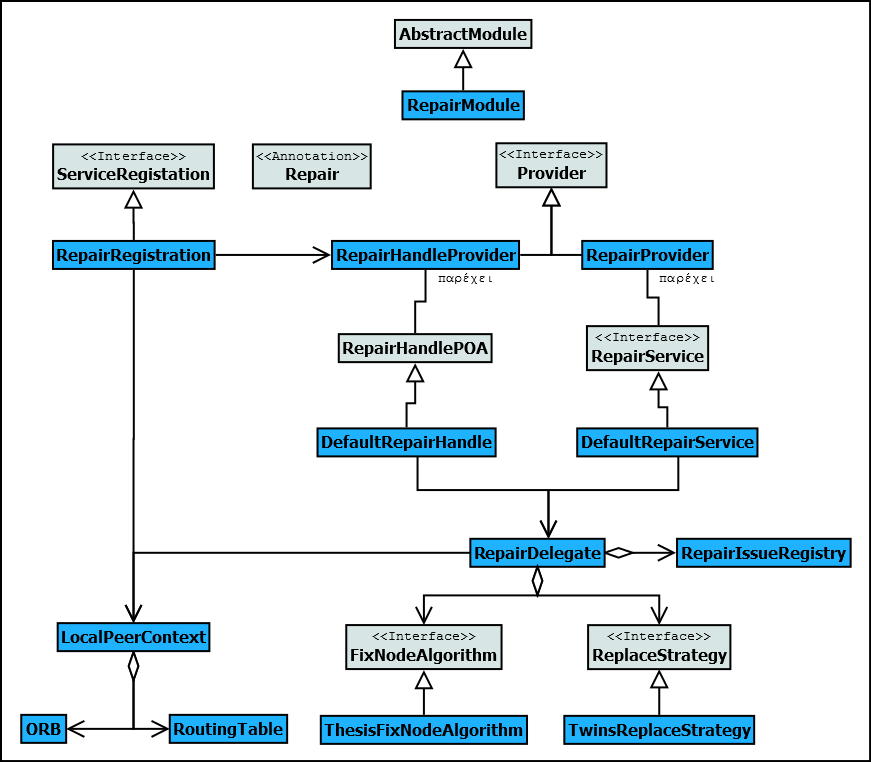
\includegraphics[width=\textwidth]{Figures/Architecture/Service_Layer/RepairService_ClassDiagram.png}
  \end{center}
  \caption{Διάγραμμα κλάσεων υπηρεσίας Repair}
  \label{fig:RepairService}
\end{figure}

Στην εικόνα \ref{fig:RepairService} φαίνεται το διάγραμμα κλάσεων της υπηρεσίας 
Repair. Αντίστοιχα με το γενικό μοντέλο της υπηρεσίας έχουμε τις 
διεπαφές RepairService και RepairHandlePOA. 

Η διεπαφή RepairService αφορά τις διεργασίες και την εφαρμογή. 
Προσφέρονται δυο μέθοδοι επιδιόρθωσης στην περίπτωση ενός αποτυχημένου 
peer ή την περίπτωση ενός αποτυχημένου υποδέντρου του δικτύου. Μετά το 
πέρας εκτέλεσης της υπηρεσίας θα έχει διορθωθεί το λάθος ή οποιοδήποτε 
αποτυχία ανακαλυφθεί στην πορεία.

Η διεπαφή RepairHandlePOA αφορά την CORBA και παράγεται μέσω της idl. Η 
υλοποίηση της φροντίζει για την αποδοχή απομακρυσμένων αιτήσεων και 
συνέχισης του αλγορίθμου.

Εδώ ακολουθούμε διαφορετική τακτική από αυτή της υπηρεσίας Exchange. Για 
την αποφυγή διπλοποίησης λειτουργικότητας και της επανάληψης κώδικα σε 
πολλά σημεία (αρχή DRY \citep{Pragmatic1999}), 
έχουμε την κλάση RepairDelegate. Σε αυτήν αναφέρονται οι υλοποιήσεις των 
διεπαφών RepairService και RepairHandlePOA για την εξυπηρέτηση των 
αιτήσεων που δέχονται. 

Παρέχονται δυο διεπαφές που αφορούν η μια τον αλγόριθμο \ref{algo:Continuation} 
FindContinuation και η άλλη την τελική διόρθωσης του προβλήματος 
από τον αλγόριθμο \ref{algo:Replace} Replace όπως έχει προκύψει από την 
ανάλυση του πρωτοκόλλου ανοχής λαθών στην ενότητα \ref{sec:Fault}. 
Και οι δυο ακολουθούν το σχεδιαστικό πρότυπο Strategy \citep{GoF}.

Συνολικά, η διεπαφή FindContinuationAlgorithm καθορίζει την κατεύθυνση που 
πρέπει να πάρει αλγόριθμος διασχίζοντας την τοπολογία του δικτύου, 
επιστρέφοντας τον κατάλληλο peer. Η διεπαφή ReplaceStrategy, 
χρησιμοποιείται όταν ο αλγόριθμος έχει καταλήξει στους δυο peer που θα 
λύσουν την αποτυχία. Η κλάση RepairDelegate περιέχει όλη την λογική που 
αφορά την επικοινωνία μεταξύ των peer για την λύση του προβλήματος. 
Επίσης, κατά την εκτέλεση της υπηρεσίας μπορεί να ανακαλυφθούν 
αποτυχημένοι peer. Κάθε ανακάλυψη αποτυχίας καταχωρείται στην 
RepairRegistry. Η RepairDelegate ελέγχει αν μπορούν να γενικευθούν 
κάποια προβλήματα από μεμονωμένους αποτυχημένους peer σε ολόκληρα 
αποτυχημένα υπόδεντρα και να καθοδηγήσει την εκτέλεση σε λύση 
υποδέντρου.

Για την κατασκευή αντικειμένων των κλάσεων που υλοποιούν τις διεπαφές 
RepairService και RepairHandlePOA υλοποιείται ο Provider. Ο RepairProvider 
προσφέρει νέα αντικείμενα τύπου RepairService σε κάθε αίτηση παροχής. 
Αντίστοιχα ο RepairHandleProvider προσφέρει το ίδιο αντικείμενο τύπου 
RepairHandlePOA. Κατά την κατασκευή και των δυο παραπάνω τύπων 
χρησιμοποιείται το ίδιο αντικείμενο τύπου RepairRegistry.

Έχουμε την υλοποίηση της διεπαφής ServiceRegistration, 
RepairRegistration, για την εγκατάσταση της υπηρεσίας την CORBA καθώς 
και το Annotation Repair χρήσιμο στην Guice.

Στην κλάση RepairModule έχουμε την παραμετροποίηση της 
υπηρεσίας, την συσχέτιση διεπαφών και υλοποιήσεων όπως φαίνονται στο 
διάγραμμα κλάσεων και την δήλωση του κύκλου ζωής των αντικειμένων.

\subsection{Υλοποίηση Υπηρεσίας Προσομοίωσης}

\begin{figure}[htbp]
  \begin{center}
    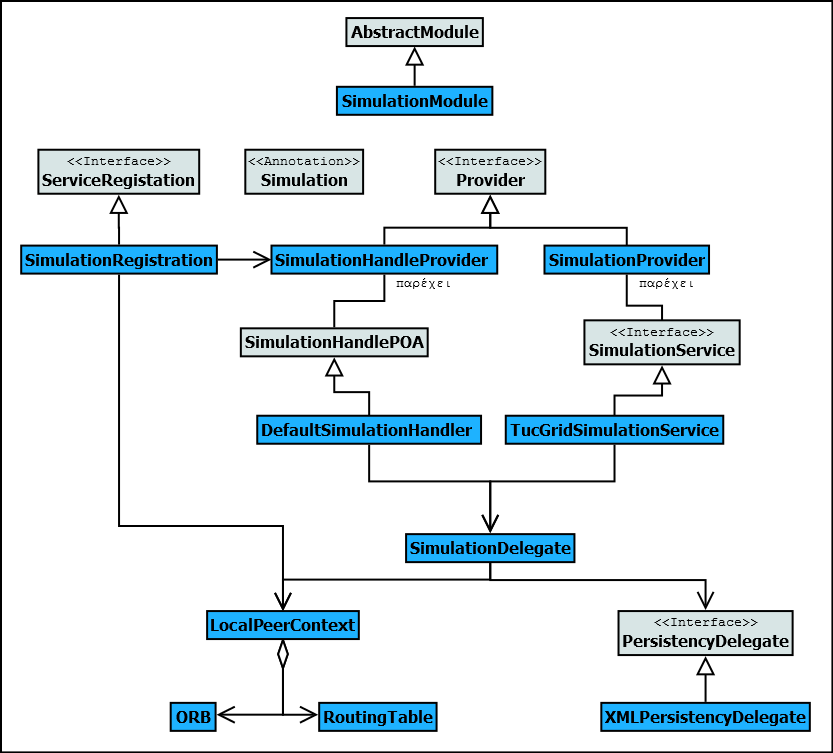
\includegraphics[width=\textwidth]{Figures/Architecture/Service_Layer/SimulationService_ClassDiagram.png}
  \end{center}
  \caption{Διάγραμμα κλάσεων υπηρεσίας Simulation}
  \label{fig:SimulationService}
\end{figure}

Για τον πειραματισμό και τον έλεγχο καλής λειτουργίας του 
συστήματος έχουμε την ανάγκη μιας υπηρεσίας που θα προσφέρει τις 
απαραίτητες λειτουργίες. Αυτό τον σκοπό εξυπηρετεί η υπηρεσία 
προσομοίωσης. 

Η υπηρεσία προσφέρει την διεπαφή SimulationProvider στις διεργασίες και 
στην εφαρμογή. Οι μέθοδοι που προσφέρει είναι:

\newcounter{numberedCntBB}
\begin{enumerate}
\item Ο τερματισμός ενός συγκεκριμένου peer. Ο peer τερματίζει χωρίς να 
ειδοποιήσει το δίκτυο και έτσι προσομοιώνεται μια αποτυχία μέσα στο 
δίκτυο.
\item Η ερώτηση για πληροφορίες ενός peer. Οι πληροφορίες περιλαμβάνουν 
τον πίνακα δρομολόγησης και το μονοπάτι στο οποίο βρίσκεται ο ερωτηθέν 
peer.
\item Ο τερματισμός της προσομοίωσης. Στην ουσία στέλνεται σήμα στο 
δίκτυο και κάθε peer τερματίζει.
\setcounter{numberedCntBB}{\theenumi}
\end{enumerate}
Στην εικόνα \ref{fig:SimulationService} φαίνεται το διάγραμμα κλάσεων 
της υπηρεσίας. Ακολουθείται η ίδια λογική με αυτή της υπηρεσίας Repair.

\subsection{Υλοποίηση Υπηρεσίας Αρχικοποίησης Συστήματος}

\begin{wrapfigure}{L}{0.42\textwidth}
  \begin{center}
    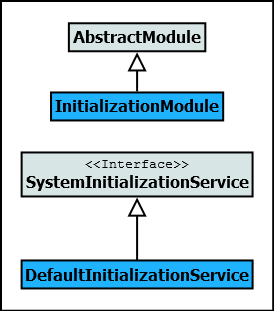
\includegraphics[width=0.40\textwidth]{Figures/Architecture/Service_Layer/InitializationService_ClassDiagram.png}
  \end{center}
  \caption{Διάγραμμα κλάσεων υπηρεσίας αρχικοποίησης}
  \label{fig:InitService}
\end{wrapfigure}

Η Guice κάνει μια μερική αρχικοποίηση του συστήματος μέσω των 
συσχετισμών που υπάρχουν μεταξύ διεπαφών και υλοποιήσεων αλλά δεν είναι 
αρκετή. Η υπηρεσία SystemInitializationService είναι υπεύθυνη για την 
πλήρη αρχικοποίηση του συστήματος. Μέσω της διεπαφής της υπηρεσίας 
μπορούν να ενεργοποιηθούν εκείνες οι υπηρεσίες που είναι απαραίτητες 
στην εφαρμογή. Επίσης, ο τοπικός peer μπορεί να αρχικοποιηθεί σε μια 
προηγούμενη κατάσταση εκτέλεσης της εφαρμογής. Αποθηκεύεται ο πίνακας 
δρομολόγησης σε μορφή XML και κατά συνέπεια μπορεί να φορτωθεί. Τέλος, 
από αυτήν την υπηρεσία ελέγχεται η εκκίνηση και ο τερματισμός της CORBA. 
Στην εικόνα \ref{fig:InitService} φαίνεται το διάγραμμα κλάσεων της υπηρεσίας. 
Παρατηρούμε πως ξεφεύγει από την γενική δομή και ο λόγος είναι η απλότητα 
της υπηρεσίας.

\section{Επίπεδο Διαδικασιών - Process Layer}

Όπως αναλύθηκε, μια σημαντική αρχή των υπηρεσιών είναι αυτή της 
σύνθεσης. Μέσω αυτής της σύνθεσης προκύπτουν οι διεργασίες οι οποίες 
ανήκουν στο παρόν επίπεδο. Στην εικόνα \ref{fig:ProcessComponent} φαίνονται 
οι διαδικασίες που περιλαμβάνονται με τις διεπαφές που εκθέτουν καθώς και τις 
εξαρτήσεις από το επίπεδο των υπηρεσιών. Οι υπάρχουσες διαδικασίες είναι 
δυο αυτή της συνάντησης δυο peer και άλλη μια που χρησιμοποιείται στην 
προσομοίωση του συστήματος.

\begin{figure}[htbp]
  \begin{center}
    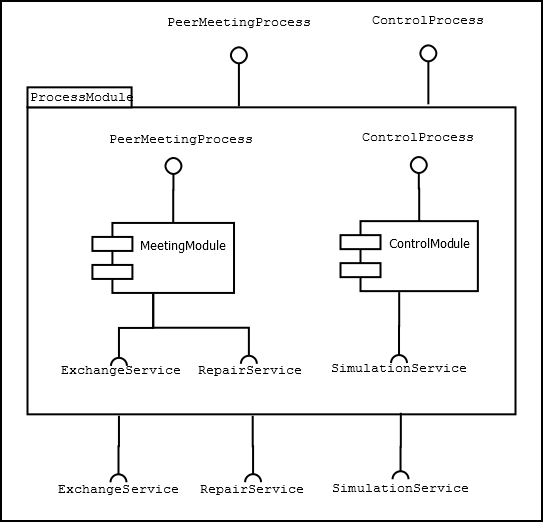
\includegraphics[width=0.6\textwidth]{Figures/Architecture/Process_Layer/Process_ComponentDiagram.png}
  \end{center}
  \caption{Διάγραμμα συστατικών επιπέδου διαδικασιών}
  \label{fig:ProcessComponent}
\end{figure}

\subsection{Διαδικασία Συνάντησης Peer}

\begin{figure}[htbp]
  \begin{center}
    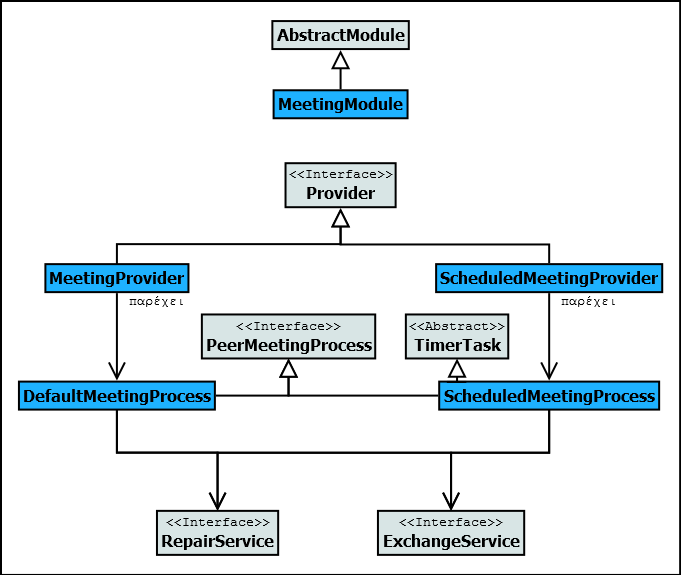
\includegraphics[width=0.85\textwidth]{Figures/Architecture/Process_Layer/MeetingProcess_ClassDiagram.png}
  \end{center}
  \caption{Διάγραμμα κλάσεων διαδικασίας συνάντησης}
  \label{fig:MeetingProcess}
\end{figure}

Η διαδικασία συνάντησης είναι τα βήματα που ακολουθούνται όταν 
ένας peer θέλει να εκτελέσει τον αλγόριθμο exchange. Κατά τον Aberer 
\citep{Abererb} σε κάθε επικοινωνία που γίνεται μεταξύ δυο peer 
εκτελείται ο αλγόριθμος. Τα βήματα που εκτελεί η διαδικασία είναι η 
εκτέλεση της υπηρεσίας ExchangeService και στην περίπτωση που έχουμε 
CommunicationException, δείγμα ότι ο απομακρυσμένος peer έχει αποτύχει, 
εκτελείται η υπηρεσία RepairService για την λύση του προβλήματος.

Η διαδικασία όπως φαίνεται στο διάγραμμα κλάσεων της στην εικόνα 
\ref{fig:MeetingProcess},ακολουθεί την γενική δομή που αναλύθηκε. 
Συγκεκριμένα, ορίζεται και παράλληλα εκτίθεται στο επίπεδο εφαρμογής 
η διεπαφή PeerMeetingProcess. Προσφέρει μια μέθοδο που θέτει σε κίνηση τα βήματα 
όπως περιγράφηκαν στην προηγούμενη παράγραφο.

Έχουμε δυο υλοποιήσεις της διεπαφής. Η πρώτη είναι μια κλασική 
υλοποίηση η οποία προορίζεται να χρησιμοποιηθεί από την εφαρμογή 
καλώντας η ίδια την διαδικασία όποτε θέλει. Η δεύτερη αφορά τον χρονικό 
προγραμματισμό της διεργασίες, ώστε να εκτελείται μετά το πέρας 
συγκεκριμένων χρονικών διαστημάτων. Αυτή επιλέγει τυχαία από τον πίνακα 
δρομολόγησης έναν peer και εκτελεί τη διαδικασία συνάντησης. Για να 
επιτευχθεί αυτό η διαδικασία επεκτείνει την κλάση TimerTask που 
προσφέρει η Java. Στη συνέχεια η εφαρμογή θα πρέπει να δημιουργήσει έναν 
Timer και να εγκαταστήσει την διαδικασία για εκτέλεση.

\subsection{Διαδικασία Ελέγχου Δικτύου}

Η διαδικασία αυτή έχει δημιουργηθεί για τον έλεγχο ενός δικτύου 
P-Grid από έναν συγκεκριμένο peer. Αποτελείται από μια κλάση την 
ControlProcess και η λειτουργικότητα που προσφέρει είναι ο εξαναγκασμός 
αποτυχίας ενός peer και η προβολή του μονοπατιού που έχουν όλοι οι peer 
του δικτύου. Να σημειωθεί πως ο peer που είναι υπεύθυνος για τον έλεγχο 
γνωρίζει όλους τους peer του δικτύου.

\chapter{Παράδειγμα Χρήσης Βιβλιοθήκης}
\label{chap:Demo}

Στην παρούσα ενότητα θα χρησιμοποιηθεί η βιβλιοθήκη για την 
προσθήκη επιπλέον υπηρεσιών και διαδικασιών. Στόχος είναι να 
παρουσιαστεί ο τρόπος και η ευκολία με την οποία μπορούν να 
κατασκευαστούν πολύπλοκες διαδικασίες με την αρχιτεκτονική που 
προτείνουμε. Επίσης, φαίνονται πώς τα χαρακτηριστικά της υπηρεσίας 
βοηθούν στο να έχουμε ανεξάρτητες και επαναχρησιμοποιήσιμες λειτουργικές 
μονάδες.

Στο σύστημα Θα προστεθεί λειτουργικότητα που αφορά τον 
διαμοιρασμό αρχείων μεταξύ των peer του δικτύου. Στις ακόλουθες 
υποενότητες θα αναλυθεί το πρόβλημα και τι προσθήκες απαιτούνται. Επίσης 
αναλύεται ο τρόπος με τον οποίο θα γίνουν αυτές οι προσθήκες.

\section{Ανάλυση Προβλήματος}

Ο στόχος όπως αναφέρθηκε είναι η προσθήκη λειτουργικότητας 
διαμοιρασμού αρχείων. Από αυτό συνεπάγεται πως ένας peer πρέπει να έχει 
μια δομή όπου θα κρατά στοιχεία για τα αρχεία τα οποία είναι 
αποθηκευμένα τοπικά. Κάθε αρχείο αντιστοιχεί σε ένα συγκεκριμένο κλειδί 
του δικτύου. Βάσει αυτού μπορεί να αναζητηθεί και να βρεθεί ο peer που 
κατέχει το αρχείο.

Πρέπει να εισαχθούν οι απαραίτητες αφαιρέσεις ώστε να 
παρουσιαστεί το δίκτυο ως ένας ενιαίος αποθηκευτικός χώρος. Βασικές 
λειτουργίες είναι η αποθήκευση ενός αρχείου στο δίκτυο και η αναζήτηση. 
Η αναζήτηση αρχείου είτε θα επιστρέψει τον κάτοχο peer σήμα ότι υπάρχει 
στο δίκτυο είτε τίποτα.

Μια βασική λειτουργία που πρέπει να υπάρχει σε ένα σύστημα διαμοιρασμού 
αρχείων είναι η δυνατότητα μεταφοράς αρχείων από μεταξύ των peer. Πέρα 
από την λήψη του αρχείου είναι απαραίτητη η αναφορά προόδου λήψης καθώς 
και η κατάσταση της (ανενεργό, αναμονή, λήψη). 

\begin{figure}[htbp]
  \begin{center}
    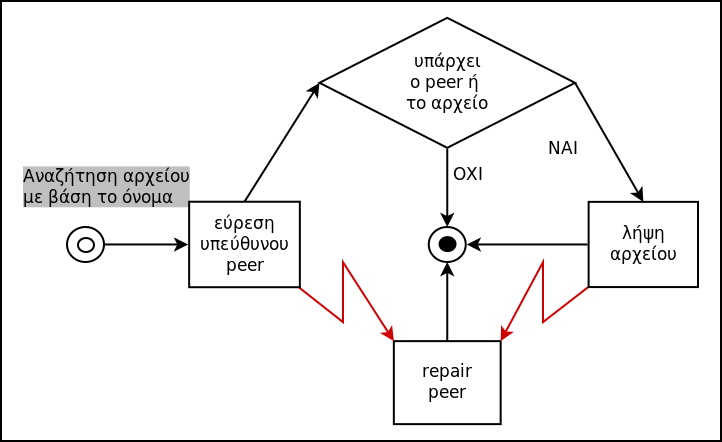
\includegraphics[width=0.9\textwidth]{Figures/Demo/Workflow.png}
  \end{center}
  \caption{Διάγραμμα ροής αναζήτησης και λήψης αρχείου}
  \label{fig:Workflow}
\end{figure}

Τέλος η διαδικασία που είναι άμεσα χρήσιμη στο επίπεδο εφαρμογής 
είναι η αναζήτηση ενός αρχείου και η λήψη του σε περίπτωση που υπάρχει. 
Στην εικόνα \ref{fig:Workflow} φαίνεται το διάγραμμα ροής αυτής της 
διεργασίας. Σε περίπτωση που ανακαλυφθεί μια αποτυχία κατά την εκτέλεση 
της τότε αυτή πρέπει να επιλυθεί.

\section{Υλοποίηση}

Από την προηγούμενη ανάλυση διακρίνουμε δύο υπηρεσίες που αφορούν τον 
αποθηκευτικό χώρο του δικτύου (Storage Service) και την μεταφορά αρχείων 
μεταξύ των peer (File Transfer Service). Η σύνθεση αυτών των δυο 
συνιστούν την διαδικασία αναζήτησης και λήψης (Download File Process). 
Για απλότητα σε κάθε peer υπάρχει ένας φάκελος όπου χρησιμοποιείται ως 
αποθηκευτικός χώρος για τα διαμοιραζόμενα αρχεία και άλλος ένας φάκελος 
όπου αποθηκεύονται τα αρχεία που από την υπηρεσία λήψης.

Σύμφωνα με την ανάλυση της αρχιτεκτονικής για να προστεθούν οι υπηρεσίες 
στο σύστημα αρκεί να υλοποιηθούν τρεις συγκεκριμένες διεπαφές/κλάσεις. Η 
κλάση AbstractModule περιγράφει την παραμετροποίηση της υπηρεσίας, ποιες 
υλοποιήσεις αντιστοιχούν σε ποιες διεπαφές. Η διεπαφή Provider είναι 
απαραίτητη για την παροχή αντικειμένων της υπηρεσίας. Μάλιστα, μέσω των 
Provider καθορίζεται και ο κύκλος ζωής της. Ο τρόπος αρχικοποίησης και 
εγκατάστασης της υπηρεσίας στο σύστημα γίνεται δια μέσου της διεπαφής 
ServiceRegistration. Τέλος, είναι αναγκαίο ο ορισμός ενός annotation ο 
οποίος χρησιμοποιείται για τον καθορισμό ποιας υλοποίησης της 
ServiceRegistration θα χρησιμοποιηθεί δεδομένου ότι υπάρχουν και άλλες 
υπηρεσίες.

Από εκεί και πέρα χρειάζεται μια διεπαφή που θα περιγράφει και θα 
εκθέτει την λειτουργικότητα της υπηρεσίας. Απαιτείται η υλοποίηση του 
κομματιού που αφορά την CORBA. Τέλος, εσωτερικά σε κάθε module υπηρεσίας 
χρειάζεται να ακολουθηθεί μια δομή όπου θα διευκολύνει την επέκταση και 
την τροποποίηση της συμπεριφοράς αυτής.

\begin{figure}[htbp]
  \begin{center}
    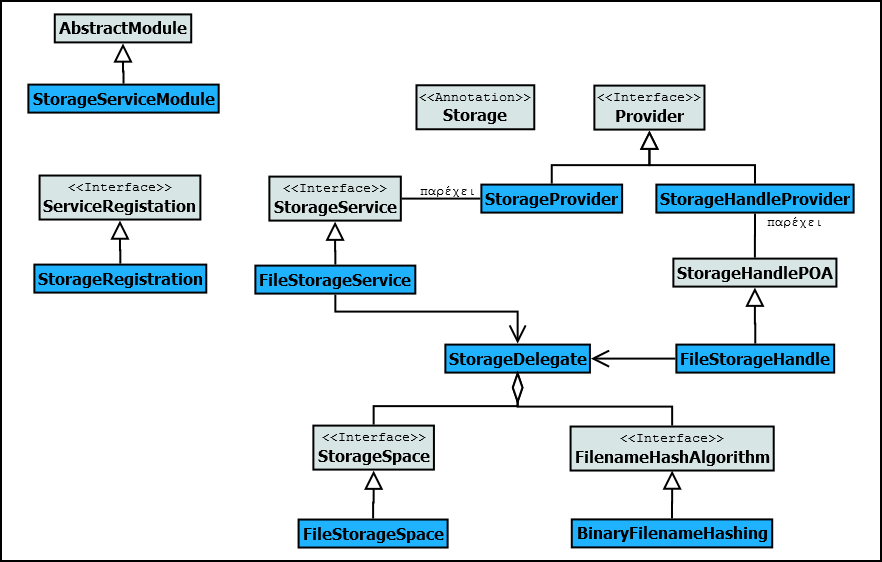
\includegraphics[width=0.95\textwidth]{Figures/Demo/StorageService_ClassDiagram.png}
  \end{center}
  \caption{Διάγραμμα κλάσεων υπηρεσίας StorageService}
  \label{fig:StorageService}
\end{figure}

\paragraph{Υλοποίηση StorageService και FileTransferService.} 
Στην εικόνα \ref{fig:StorageService} φαίνεται το διάγραμμα κλάσεων 
της υπηρεσίας StorageService. Μπορούμε να δούμε τα αντικείμενα που 
υλοποιούν ή επεκτείνουν τις απαραίτητες διεπαφές/κλάσεις όπως έχει 
περιγραφεί παραπάνω. Οι κλάσεις StorageHandlePOA έχει παραχθεί από 
την idl και αφορά την CORBA. Παρέχεται Provider και για αυτή την 
διεπαφή. Στην εικόνα \ref{fig:FileTransferService} φαίνεται το 
διάγραμμα κλάσεων της υπηρεσίας FileTransferService. Ακολουθείται 
αντίστοιχη λογική.

\begin{figure}[htbp]
  \begin{center}
    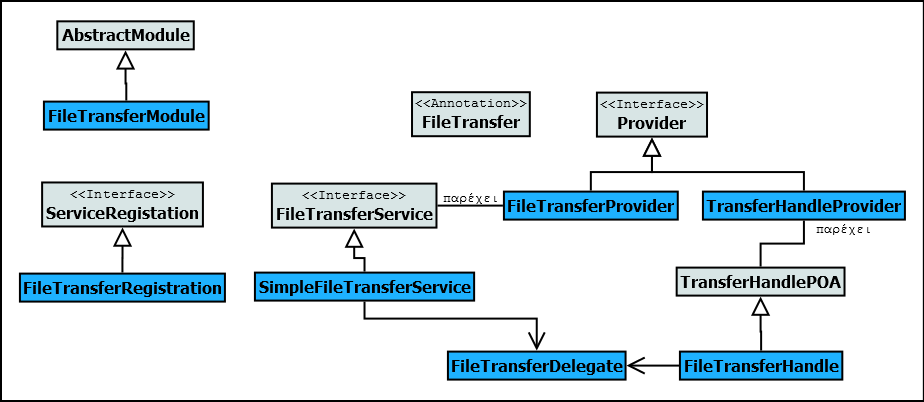
\includegraphics[width=0.95\textwidth]{Figures/Demo/FileTransferService_ClassDiagram.png}
  \end{center}
  \caption{Διάγραμμα κλάσεων υπηρεσίας FileTransferService}
  \label{fig:FileTransferService}
\end{figure}

\paragraph{Υλοποίηση DownloadFileProcess.}
Αυτό που μένει είναι η υλοποίηση της διαδικασίας 
DownloadFileProcess. Το διάγραμμα κλάσεων φαίνεται στην εικόνα 
\ref{fig:DownloadFileProcess}. Φαίνεται και η χρήση της υπηρεσίας 
επιδιόρθωσης RepairService που καταστά την διαδικασία fault-tolerant.

\begin{figure}[htbp]
  \begin{center}
    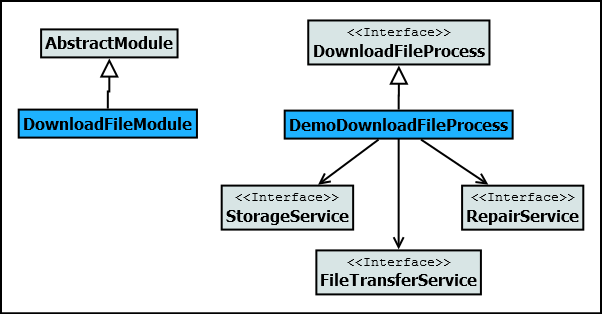
\includegraphics[width=0.9\textwidth]{Figures/Demo/DownloadFileProcess_ClassDiagram.png}
  \end{center}
  \caption{Διάγραμμα κλάσεων διαδικασίας DownloadFileProcess}
  \label{fig:DownloadFileProcess}
\end{figure}

Στην εικόνα \ref{fig:DownloadFile_Sequence} φαίνεται το διάγραμμα 
ακολουθίας της διαδικασία όταν καλείται από τον χρήστη. Φαίνεται ξεκάθαρα 
πώς τα αντικείμενα σε επίπεδο διαδικασίας αλληλεπιδρούν. Συγκεκριμένα φαίνεται 
η περίπτωση όπου το αρχείο υπάρχει σε κάποιον peer το δικτύου ο οποίος 
και επιστρέφεται όταν τερματίζει η εκτέλεση της υπηρεσίας 
StorageService. Η διαδικασία επιστρέφει στον χρήστη την κατάσταση στην 
οποία τερμάτισε. Οι καταστάσεις που έχουν οριστεί στην διεπαφή είναι 
FILE\_NOT\_FOUND, NETWORK\_ERROR και FILE\_DOWNLOADED. Επίσης, φαίνεται 
και ο κύκλος ζωής των υπηρεσιών αυτών. Σε νέα αίτηση θα κατασκευαστούν 
εκ νέου τα αντικείμενα. Κάτι αντίστοιχο συμβαίνει όταν ο peer δέχεται 
αιτήσεις για εξυπηρέτηση υπηρεσιών. Η διαφορά είναι ότι εκεί τα 
αντικείμενα που αφορούν την CORBA είναι ίδια μέχρι τον τερματισμό του 
peer.

\begin{figure}[htbp]
  \begin{center}
    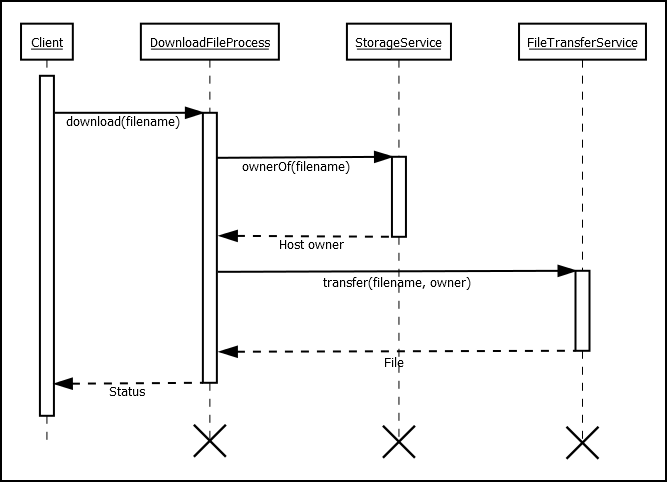
\includegraphics[width=0.9\textwidth]{Figures/Demo/DownloadFileProcess_Sequence.png}
  \end{center}
  \caption{Διάγραμμα ακολουθίας της διαδικασίας DownloadFileProcess}
  \label{fig:DownloadFile_Sequence}
\end{figure}

\chapter{Επίλογος}
\label{chap:Closing}

\section{Συμπεράσματα}

\ \ \ \ TODO

\section{Μελλοντική Εργασία}

\ \ \ \ TODO


%% ----------------------------------------------------------------
\label{Bibliography}
\bibliographystyle{unsrtnat}  % formatting the Bibliography
\bibliography{Bibliography}

\end{document}
%% ----------------------------------------------------------------
